\section{Introduzione al corso} % (fold)
\label{sec:intro}
% Local background must be enclosed by curly braces for grouping.
{
    \usebackgroundtemplate{\includegraphics[width=\paperwidth]{IMG_0066_scaled_128_96.png}}
    \begin{frame}[t, fragile] \frametitle{Chi?}
    \framesubtitle{\phantom{\_}}
        \vspace*{-5pt}
        \hspace*{-13pt}
        {\huge
            \color{white} \faUser\ \textbf{Simone Scannapieco}
        }
        {
            \begin{itemize}[leftmargin=10pt,align=right]
                \setlength\itemsep{.7em}
                \item[\color{white}\faBook] \color{white} Ph.D. in Informatica (Metodi formali e AI)
                \item[\color{white}\faBriefcase] \color{white} Ricercatore AI e sviluppatore
                \item[\color{white}\faCodeFork] \color{white} AI \emph{engineer} (mai dire esperto\ldots)
                \item[\color{white}\faCameraRetro] \color{white} Disegnatore di luce
                \item[\color{white}\faBicycle] \color{white} Amante delle due ruote
                \item[\color{white}\faLinkedin] \color{white} \href{https://www.linkedin.com/in/simonescannapieco/}{\color{venis-faithful-yellow}\texttt{simonescannapieco}}
            \end{itemize}
        }
    \end{frame}
}
%
\begin{frame}[t,fragile] \frametitle{Quando?}
\framesubtitle{Cronoprogramma del corso}
    \begin{itemize}[leftmargin=10pt,align=right]
        \onslide<1->\item[\alert{\faArrowCircleRight}] 28 ore totali
        \onslide<2->\item[\alert{\faArrowCircleRight}] Date
        \begin{itemize}[leftmargin=10pt,align=right]
            \item[\alert{\faArrowCircleRight}] 23 Settembre 2025
            \item[\alert{\faArrowCircleRight}] 25 Settembre 2025
            \item[\alert{\faArrowCircleRight}] 07 Ottobre 2025
            \item[\alert{\faArrowCircleRight}] 09 Ottobre 2025
        \end{itemize}
        \onslide<3->\item[\alert{\faArrowCircleRight}] Orari
        \begin{itemize}[leftmargin=10pt,align=right]
            \item[\alert{\faArrowCircleRight}] 9:00 - 13:00; 14:00 - 17:00
        \end{itemize}
    \end{itemize}
    \onslide<4->
    \begin{center}
        \begin{minipage}[b]{.45\textwidth}
		    \begin{figure}[ht]
			    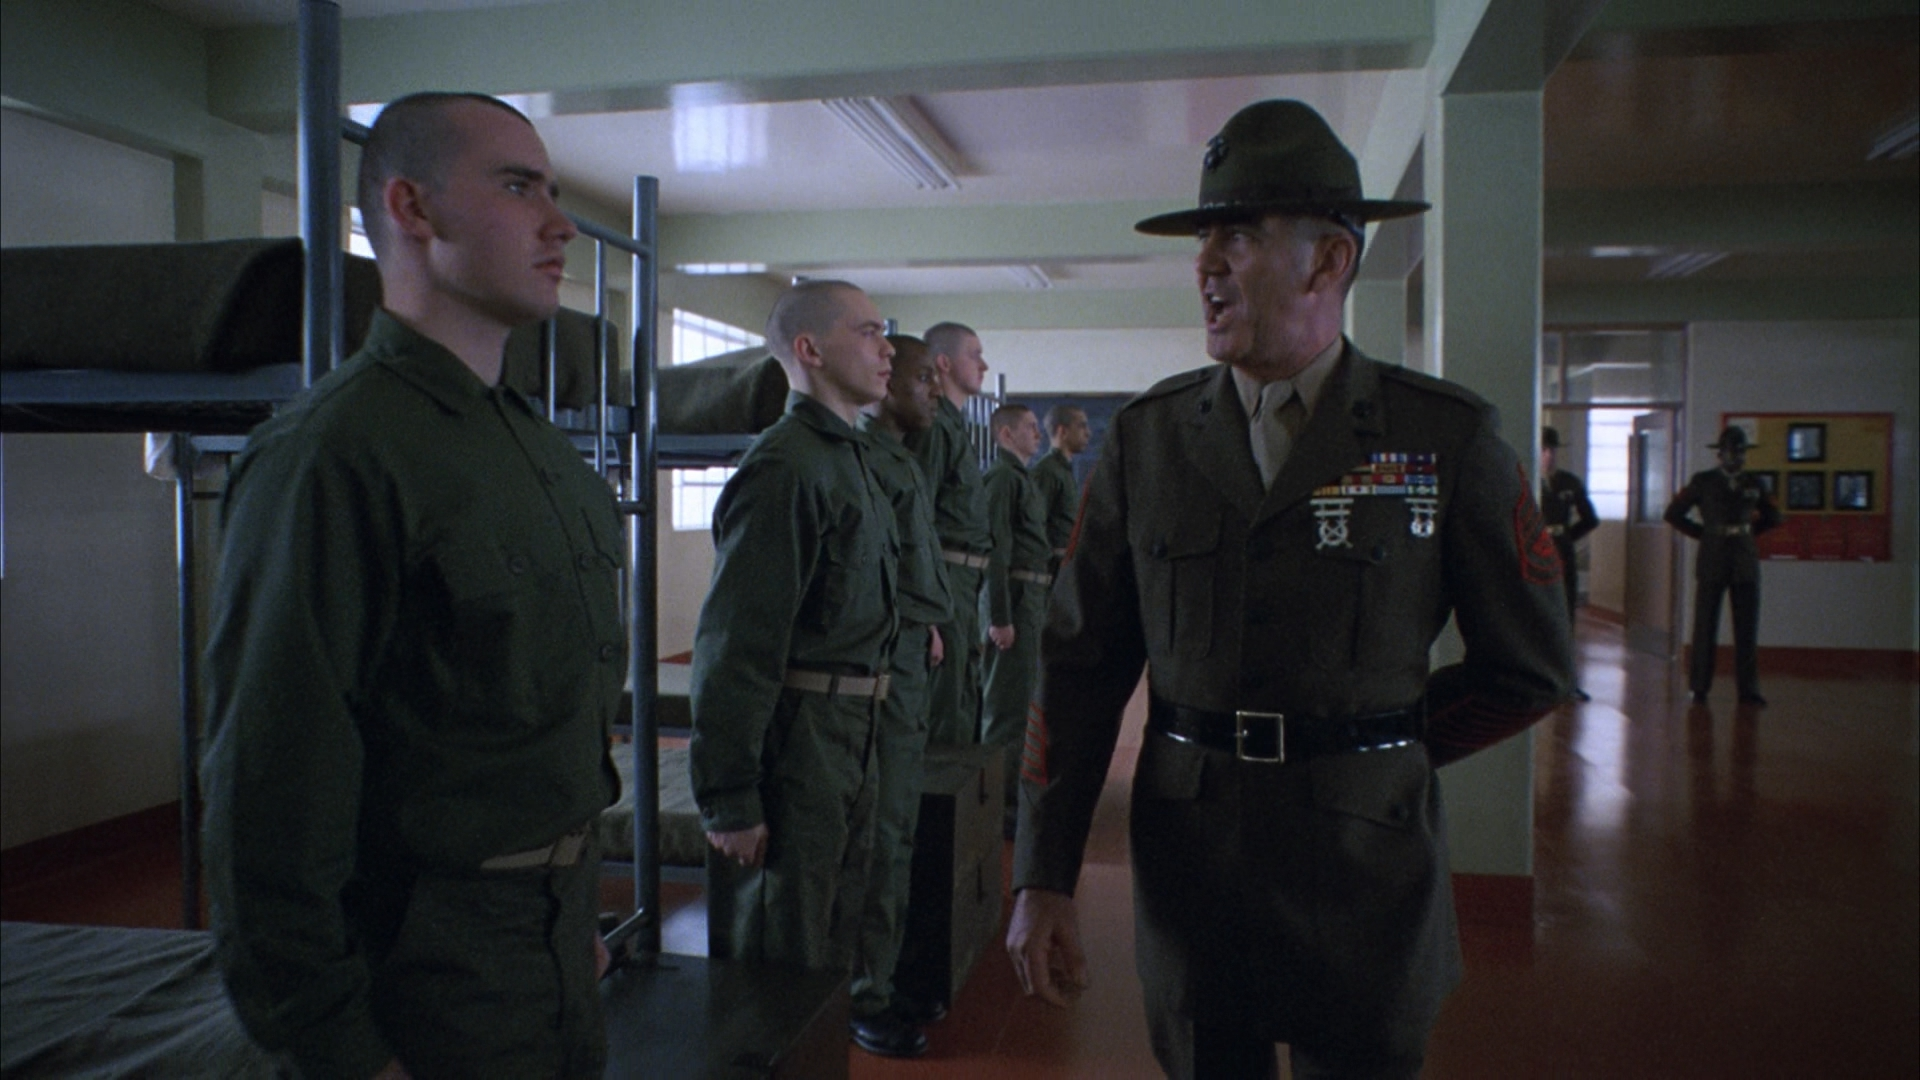
\includegraphics[width=\textwidth]{full-metal-jacket.jpg}
		    \end{figure}
            \begin{flushright}
                \vspace*{-10pt}
                {\tiny\textit{\textcopyright Wikimedia Creative Commons}}
            \end{flushright}
	    \end{minipage}
    \end{center}
\end{frame}
%
\begin{frame}[t,fragile] \frametitle{Come?}
\framesubtitle{Tecnologie, IDEs, linguaggi}
\begin{itemize}[leftmargin=10pt,align=right]
    \setlength\itemsep{.7em}
    \onslide<1->\item[\alert{\faArrowCircleRight}] Linguaggi e librerie principali
    \onslide<2->\begin{minipage}[t]{\textwidth}
        \begin{minipage}[t]{.2\textwidth}
            \begin{figure}[ht]
                
\includegraphics[height=20pt,keepaspectratio]{java.png}
            \end{figure}
        \end{minipage}
    \end{minipage}
    \onslide<3->\item[\alert{\faArrowCircleRight}] \emph{Frameworks}
    \onslide<4->\begin{minipage}[t]{\textwidth}
        \begin{minipage}[t]{.2\textwidth}
            \begin{figure}[ht]
                
\includegraphics[height=20pt,keepaspectratio]{spring-boot.png}
            \end{figure}
        \end{minipage}
        \begin{minipage}[t]{.2\textwidth}
            \begin{figure}[ht]
                
\includegraphics[height=20pt,keepaspectratio]{spring-ai-cut.png}
            \end{figure}
        \end{minipage}
    \end{minipage}
    \onslide<5->\item[\alert{\faArrowCircleRight}] Servizi AI e modelli
    \onslide<6->\begin{minipage}[t]{\textwidth}
        \begin{minipage}[t]{.2\textwidth}
            \begin{figure}[ht]
                
\includegraphics[height=20pt,keepaspectratio]{openai-cut.png}
            \end{figure}
        \end{minipage}
        \begin{minipage}[t]{.2\textwidth}
            \begin{figure}[ht]
                
\includegraphics[height=20pt,keepaspectratio]{google-apis-alpha.png}
            \end{figure}
        \end{minipage}
        \begin{minipage}[t]{.2\textwidth}
            \begin{figure}[ht]
                
\includegraphics[height=20pt,keepaspectratio]{gemini.png}
            \end{figure}
        \end{minipage}
        \begin{minipage}[t]{.2\textwidth}
            \begin{figure}[ht]
                
\includegraphics[height=20pt,keepaspectratio]{ollama.png}
            \end{figure}
        \end{minipage}
    \end{minipage}
    \onslide<7->\item[\alert{\faArrowCircleRight}] IDEs
    \onslide<8->\begin{minipage}[t]{\textwidth}
        \begin{minipage}[t]{.2\textwidth}
            \begin{figure}[ht]
                
\includegraphics[height=20pt,keepaspectratio]{vscode.png}
            \end{figure}
        \end{minipage}
    \end{minipage}
\end{itemize}
\end{frame}
%
\begin{frame}[t,fragile] \frametitle{Perché?}
\only<1-2|handout:1>{\framesubtitle{Generative AI e LLM: \emph{trend} di richiesta lavorativa}}
\only<3|handout:2>{\framesubtitle{Generative AI e LLM: \emph{shift} di priorità tecnologica}}
\only<4-7|handout:3-4>{\framesubtitle{Generative AI e LLM: sulla bocca degli alti dirigenti}}
{\scriptsize
\only<1|handout:0>{
    \begin{figure}[ht]
            \centering
            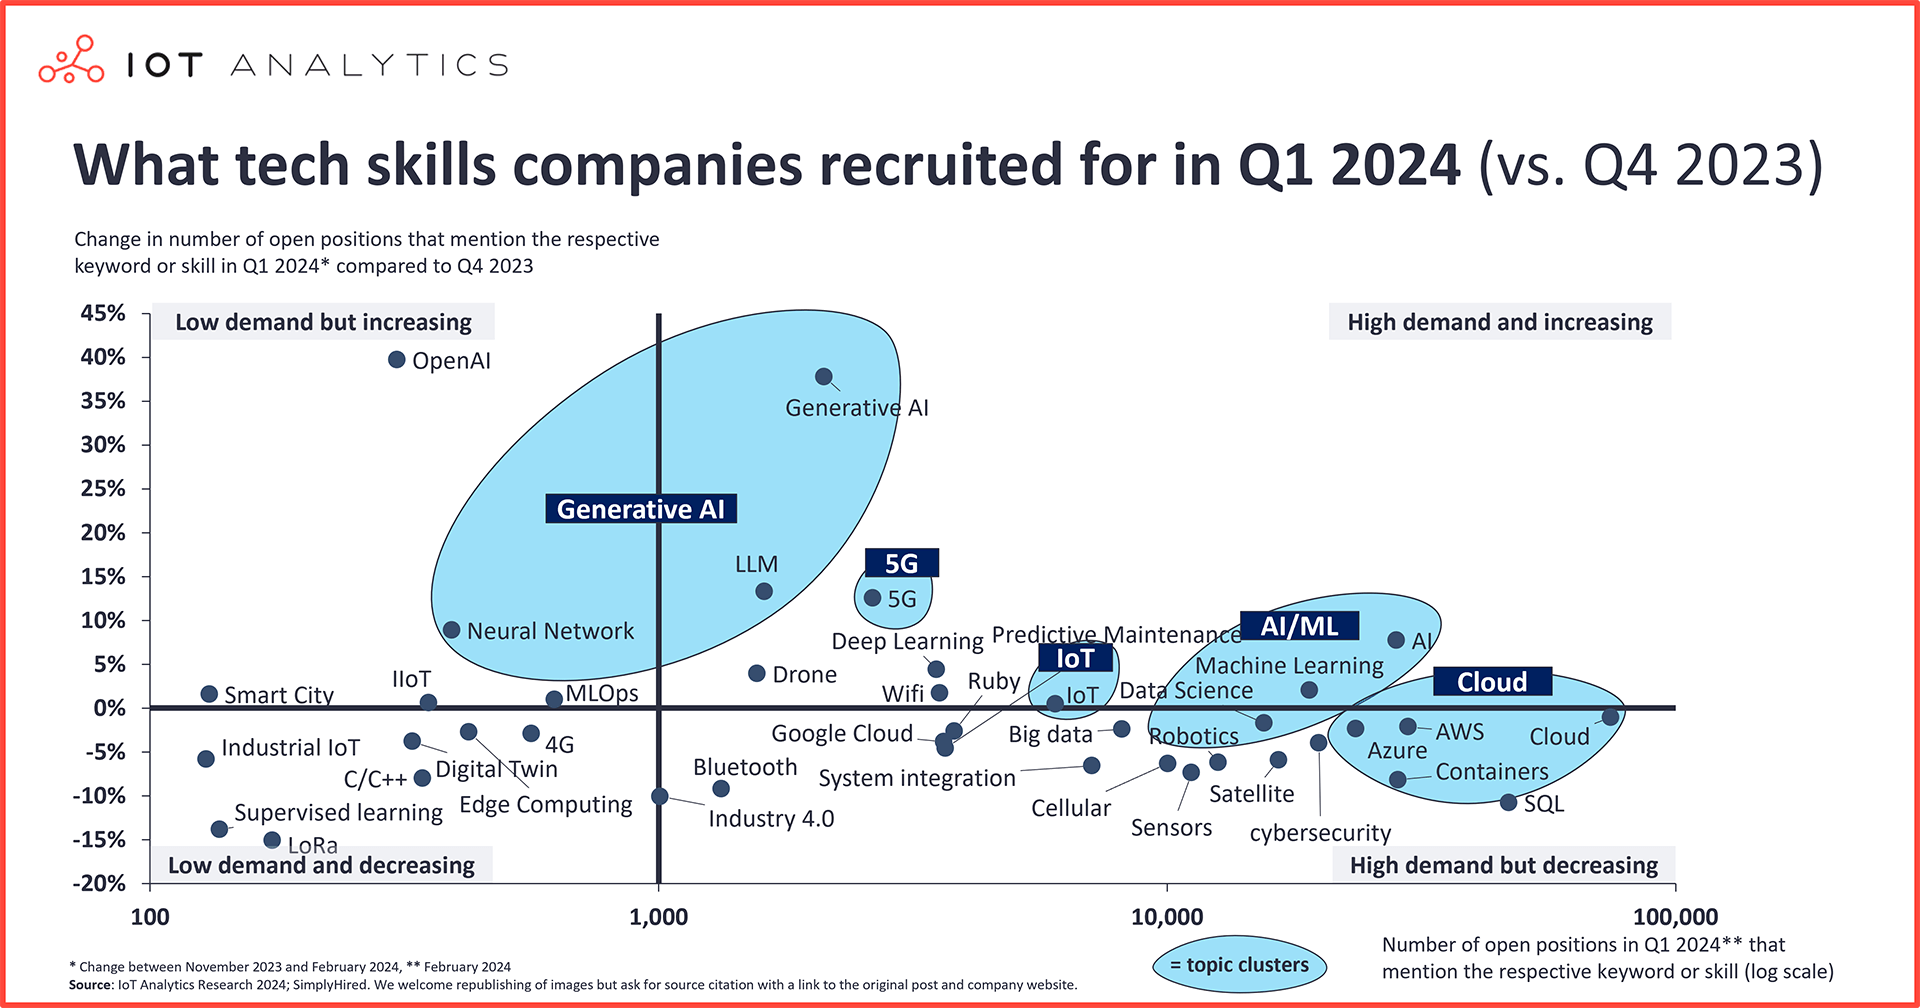
\includegraphics[width=\textwidth]{tech-skills.png}
    \end{figure}
}
\only<2|handout:1>{
    \begin{figure}[ht]
        \centering
        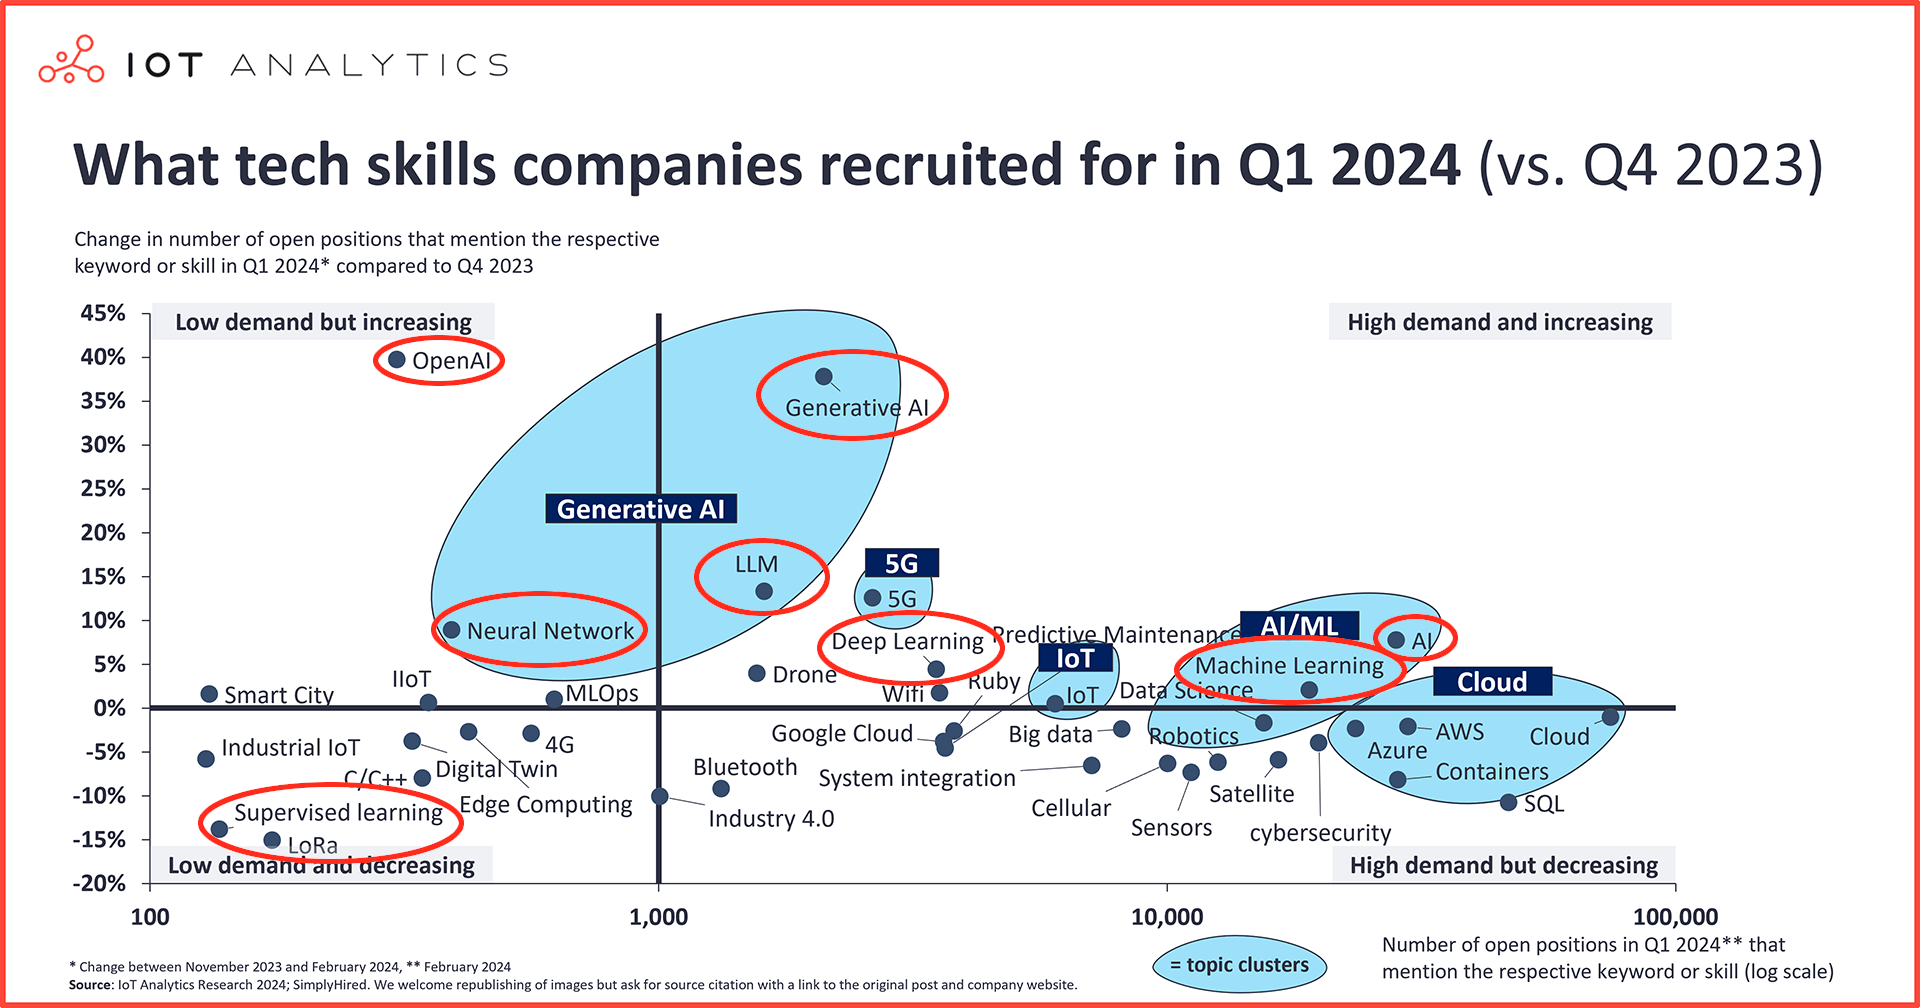
\includegraphics[width=\textwidth]{tech-skills-ellipses.png}
    \end{figure}
}
\only<3|handout:2>{
    \begin{figure}[ht]
        \centering
        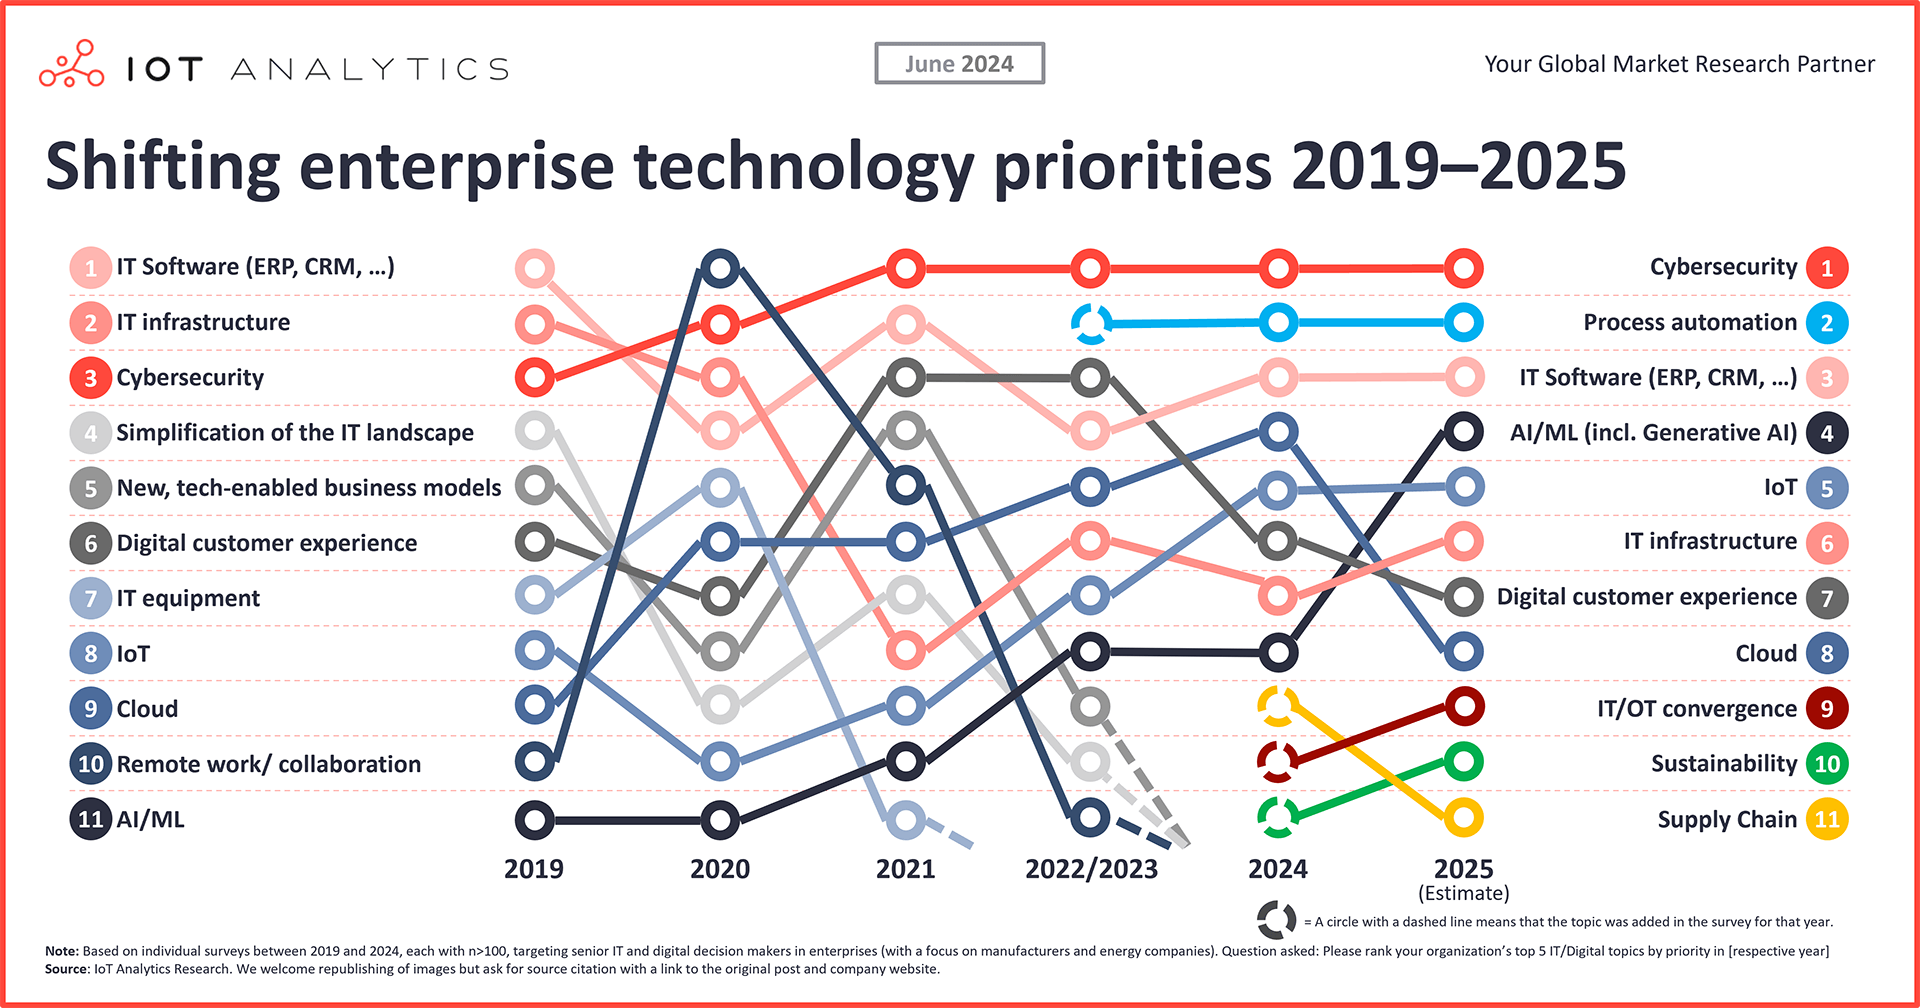
\includegraphics[width=\textwidth]{shifting-enterprise-technology-priorities.png}
    \end{figure}
}
\only<4|handout:0>{
    \begin{figure}[ht]
        \centering
        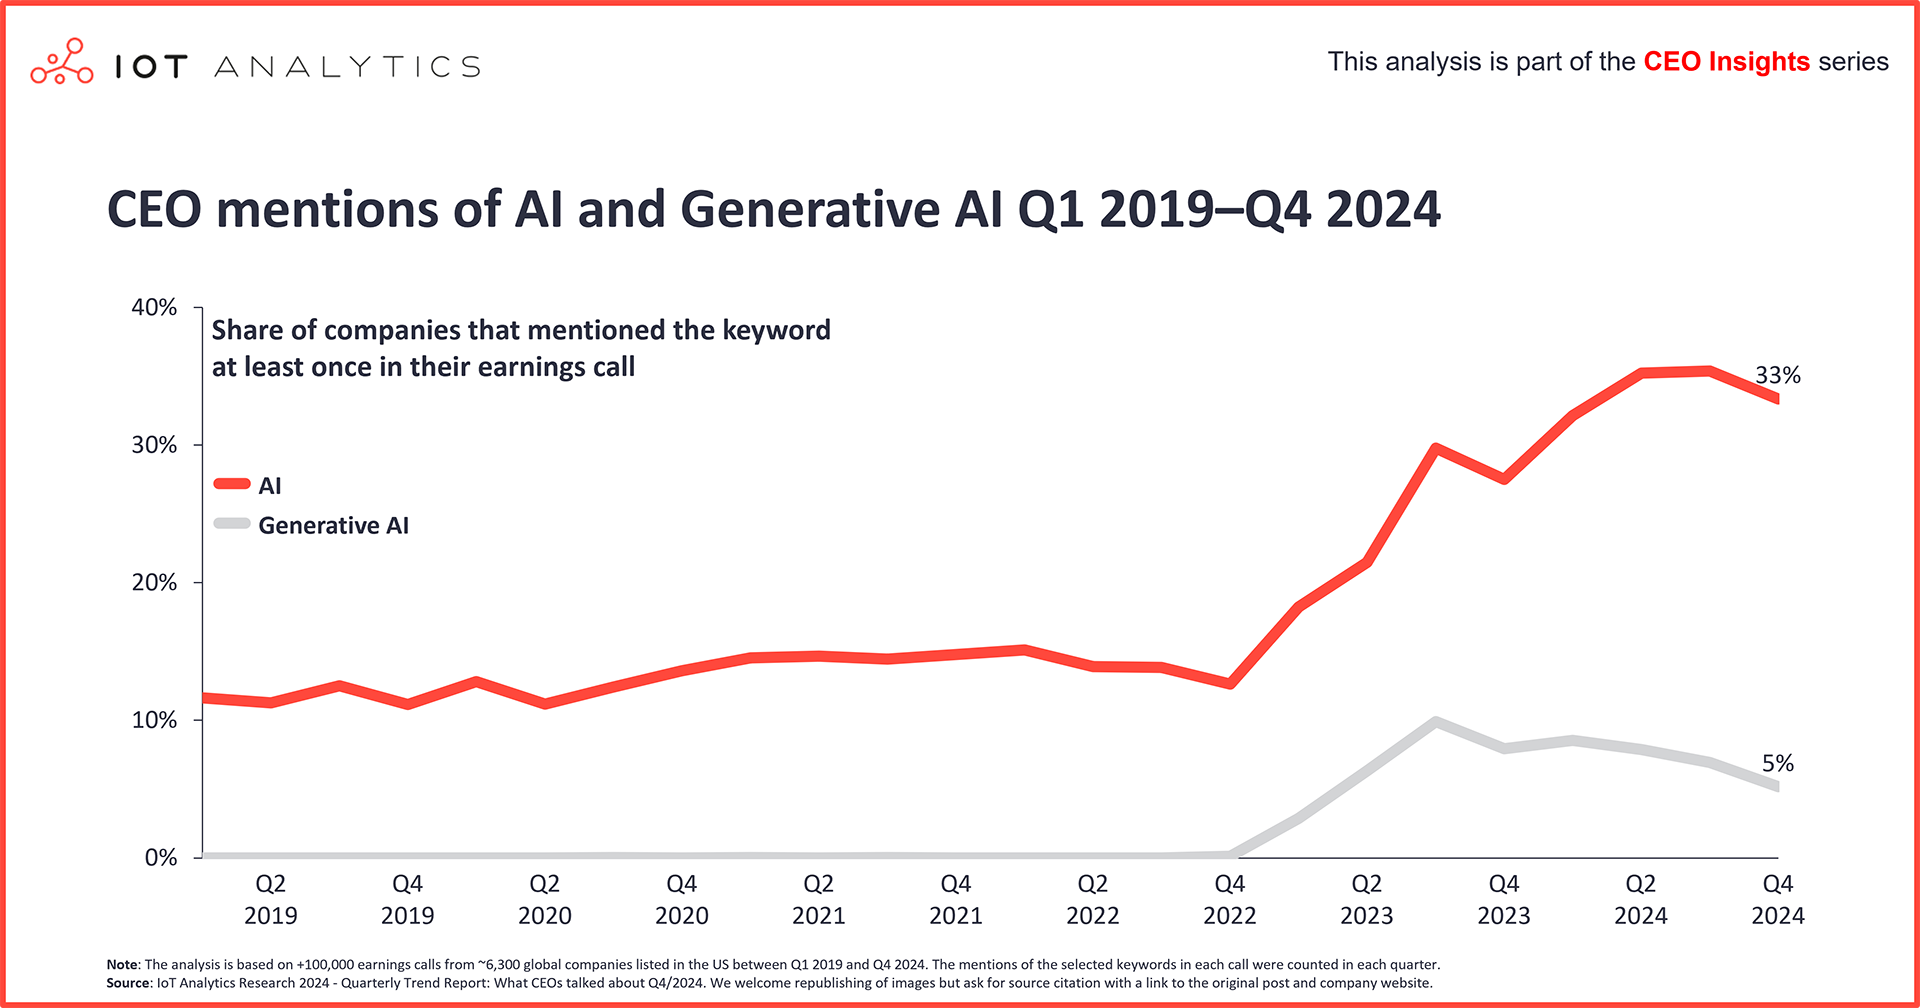
\includegraphics[width=\textwidth]{ceo-mentions-of-ai-and-generative-ai-19-24.png}
    \end{figure}
}
\only<5|handout:3>{
    \begin{figure}[ht]
        \centering
        \includegraphics[width=\textwidth]{ceo-mentions-of-ai-and-generative-ai-19-24-llms.png}
    \end{figure}
}
\only<6|handout:0>{
    \begin{figure}[ht]
        \centering
        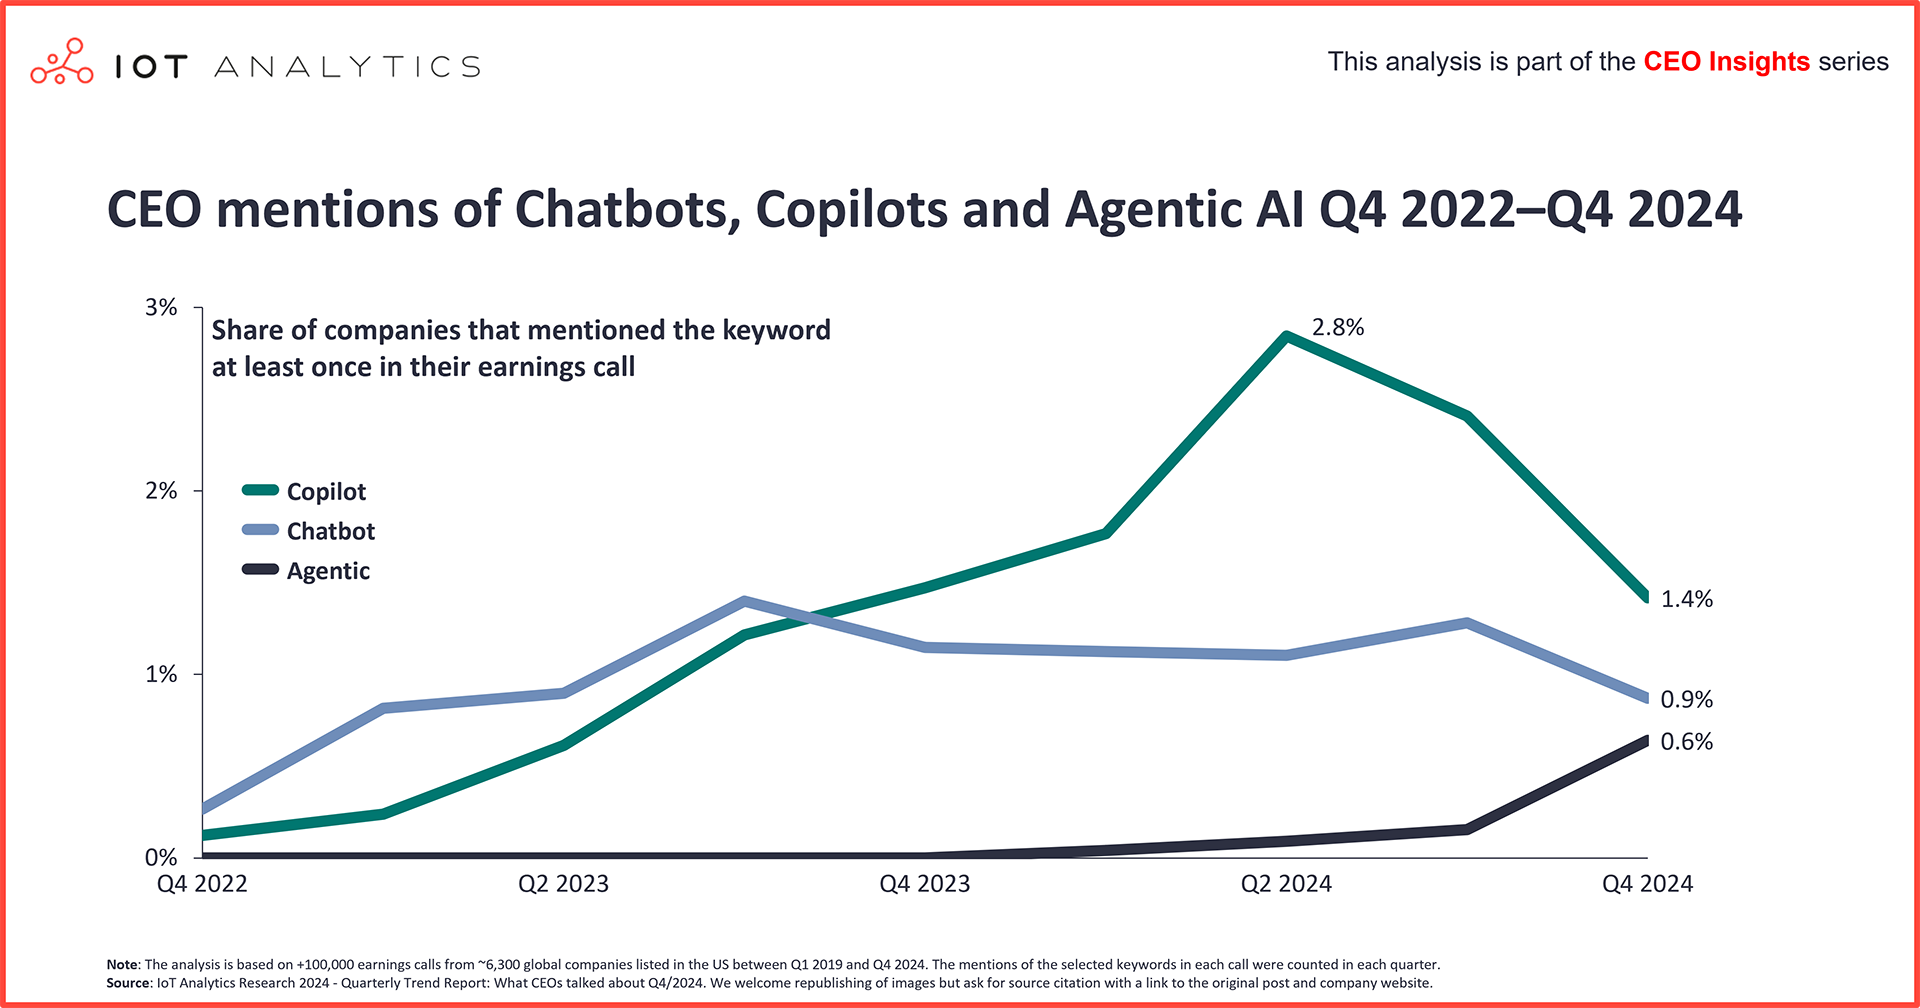
\includegraphics[width=\textwidth]{ceo-mentions-of-chatbots-copilots-and-agentic-ai-22-24.png}
    \end{figure}
}
\only<7|handout:4>{
    \begin{figure}[ht]
        \centering
        \includegraphics[width=\textwidth]{ceo-mentions-of-chatbots-copilots-and-agentic-ai-22-24-copilot-pro.png}
    \end{figure}
}
\begin{flushright}
    \vspace*{-5pt}
    \only<1-2|handout:1>{\tiny\textit{\textcopyright Philipp Wegner, IoT Analytics}}
    \only<3|handout:2>{\tiny\textit{\textcopyright Knud Lasse Lueth, IoT Analytics}}
    \only<4-7|handout:3-4>{\tiny\textit{\textcopyright Philipp Wegner, IoT Analytics}}
\end{flushright}
}
\end{frame}
%
\begin{frame}[t,fragile] \frametitle{Perché?}
\framesubtitle{Lezioni che (spero) impariate}
{\scriptsize
    \begin{minipage}[b]{\textwidth}
        \onslide<2->
        \begin{minipage}[b]{0.33\textwidth}
            \centering
            \begin{figure}[ht]
                
\includegraphics[width=\textwidth]{meme-2.jpg}
            \end{figure}
            \begin{flushright}
                \vspace*{-7pt}
                {\tiny\textit{\textcopyright imgflip.com}}
            \end{flushright}
        \end{minipage}
        \onslide<3->
        \begin{minipage}[b]{0.33\textwidth}
            \centering
            \begin{figure}[ht]
                
\includegraphics[width=\textwidth]{meme-3-cut.jpeg}
            \end{figure}
            \begin{flushright}
                \vspace*{-7pt}
                {\tiny\textit{\textcopyright imgflip.com}}
            \end{flushright}
        \end{minipage}
        \onslide<4->
        \begin{minipage}[b]{0.33\textwidth}
            \centering
            \begin{figure}[ht]
                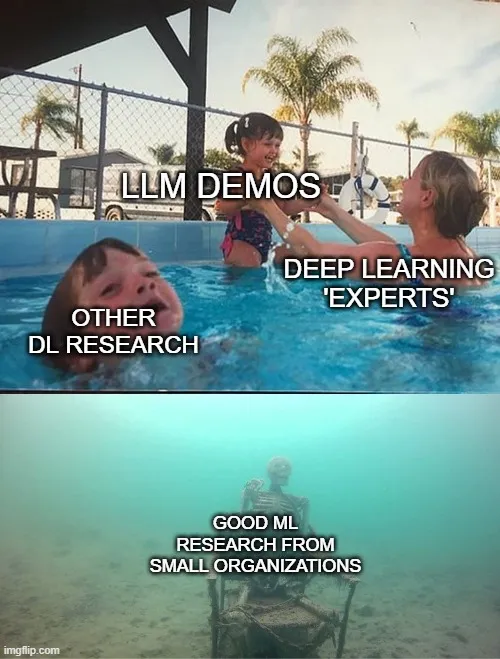
\includegraphics[width=\textwidth]{meme-1.png}
            \end{figure}
            \begin{flushright}
                \vspace*{-7pt}
                {\tiny\textit{\textcopyright imgflip.com}}
            \end{flushright}
        \end{minipage}
    \end{minipage}
    \begin{itemize}[leftmargin=10pt,align=right]
        \onslide<2->\item[\alert{\faArrowCircleRight}] Capire cosa si intende per AI, ML e DL
        \onslide<3->\item[\alert{\faArrowCircleRight}] GENAI e LLM sono il \textit{trend} del momento
        \begin{itemize}[leftmargin=10pt,align=right]
            \onslide<3->\item[\alert{\faArrowCircleRight}] Tutti ne parlano, tutti sono esperti
            \onslide<4->\item[\alert{\faArrowCircleRight}] \alert{Non} è la panacea di tutti i mali
            \onslide<4->\item[\alert{\faArrowCircleRight}] A volte, approcci meno complessi sono sufficienti
        \end{itemize}
    \end{itemize}
}
\end{frame}
%
\begin{frame}[t,fragile] \frametitle{Cosa?}
	\framesubtitle{Da AI a LLMs}
	{\scriptsize
	    \only<1|handout:0>{
	    \begin{figure}[ht]
                \begin{minipage}[b]{0.95\linewidth}
                    \centering
                    
\includegraphics[width=\textwidth]{1.png}
                \end{minipage}
            \end{figure}
        }
        \only<2|handout:0>{
	    \begin{figure}[ht]
                \begin{minipage}[b]{0.95\linewidth}
                    \centering
                    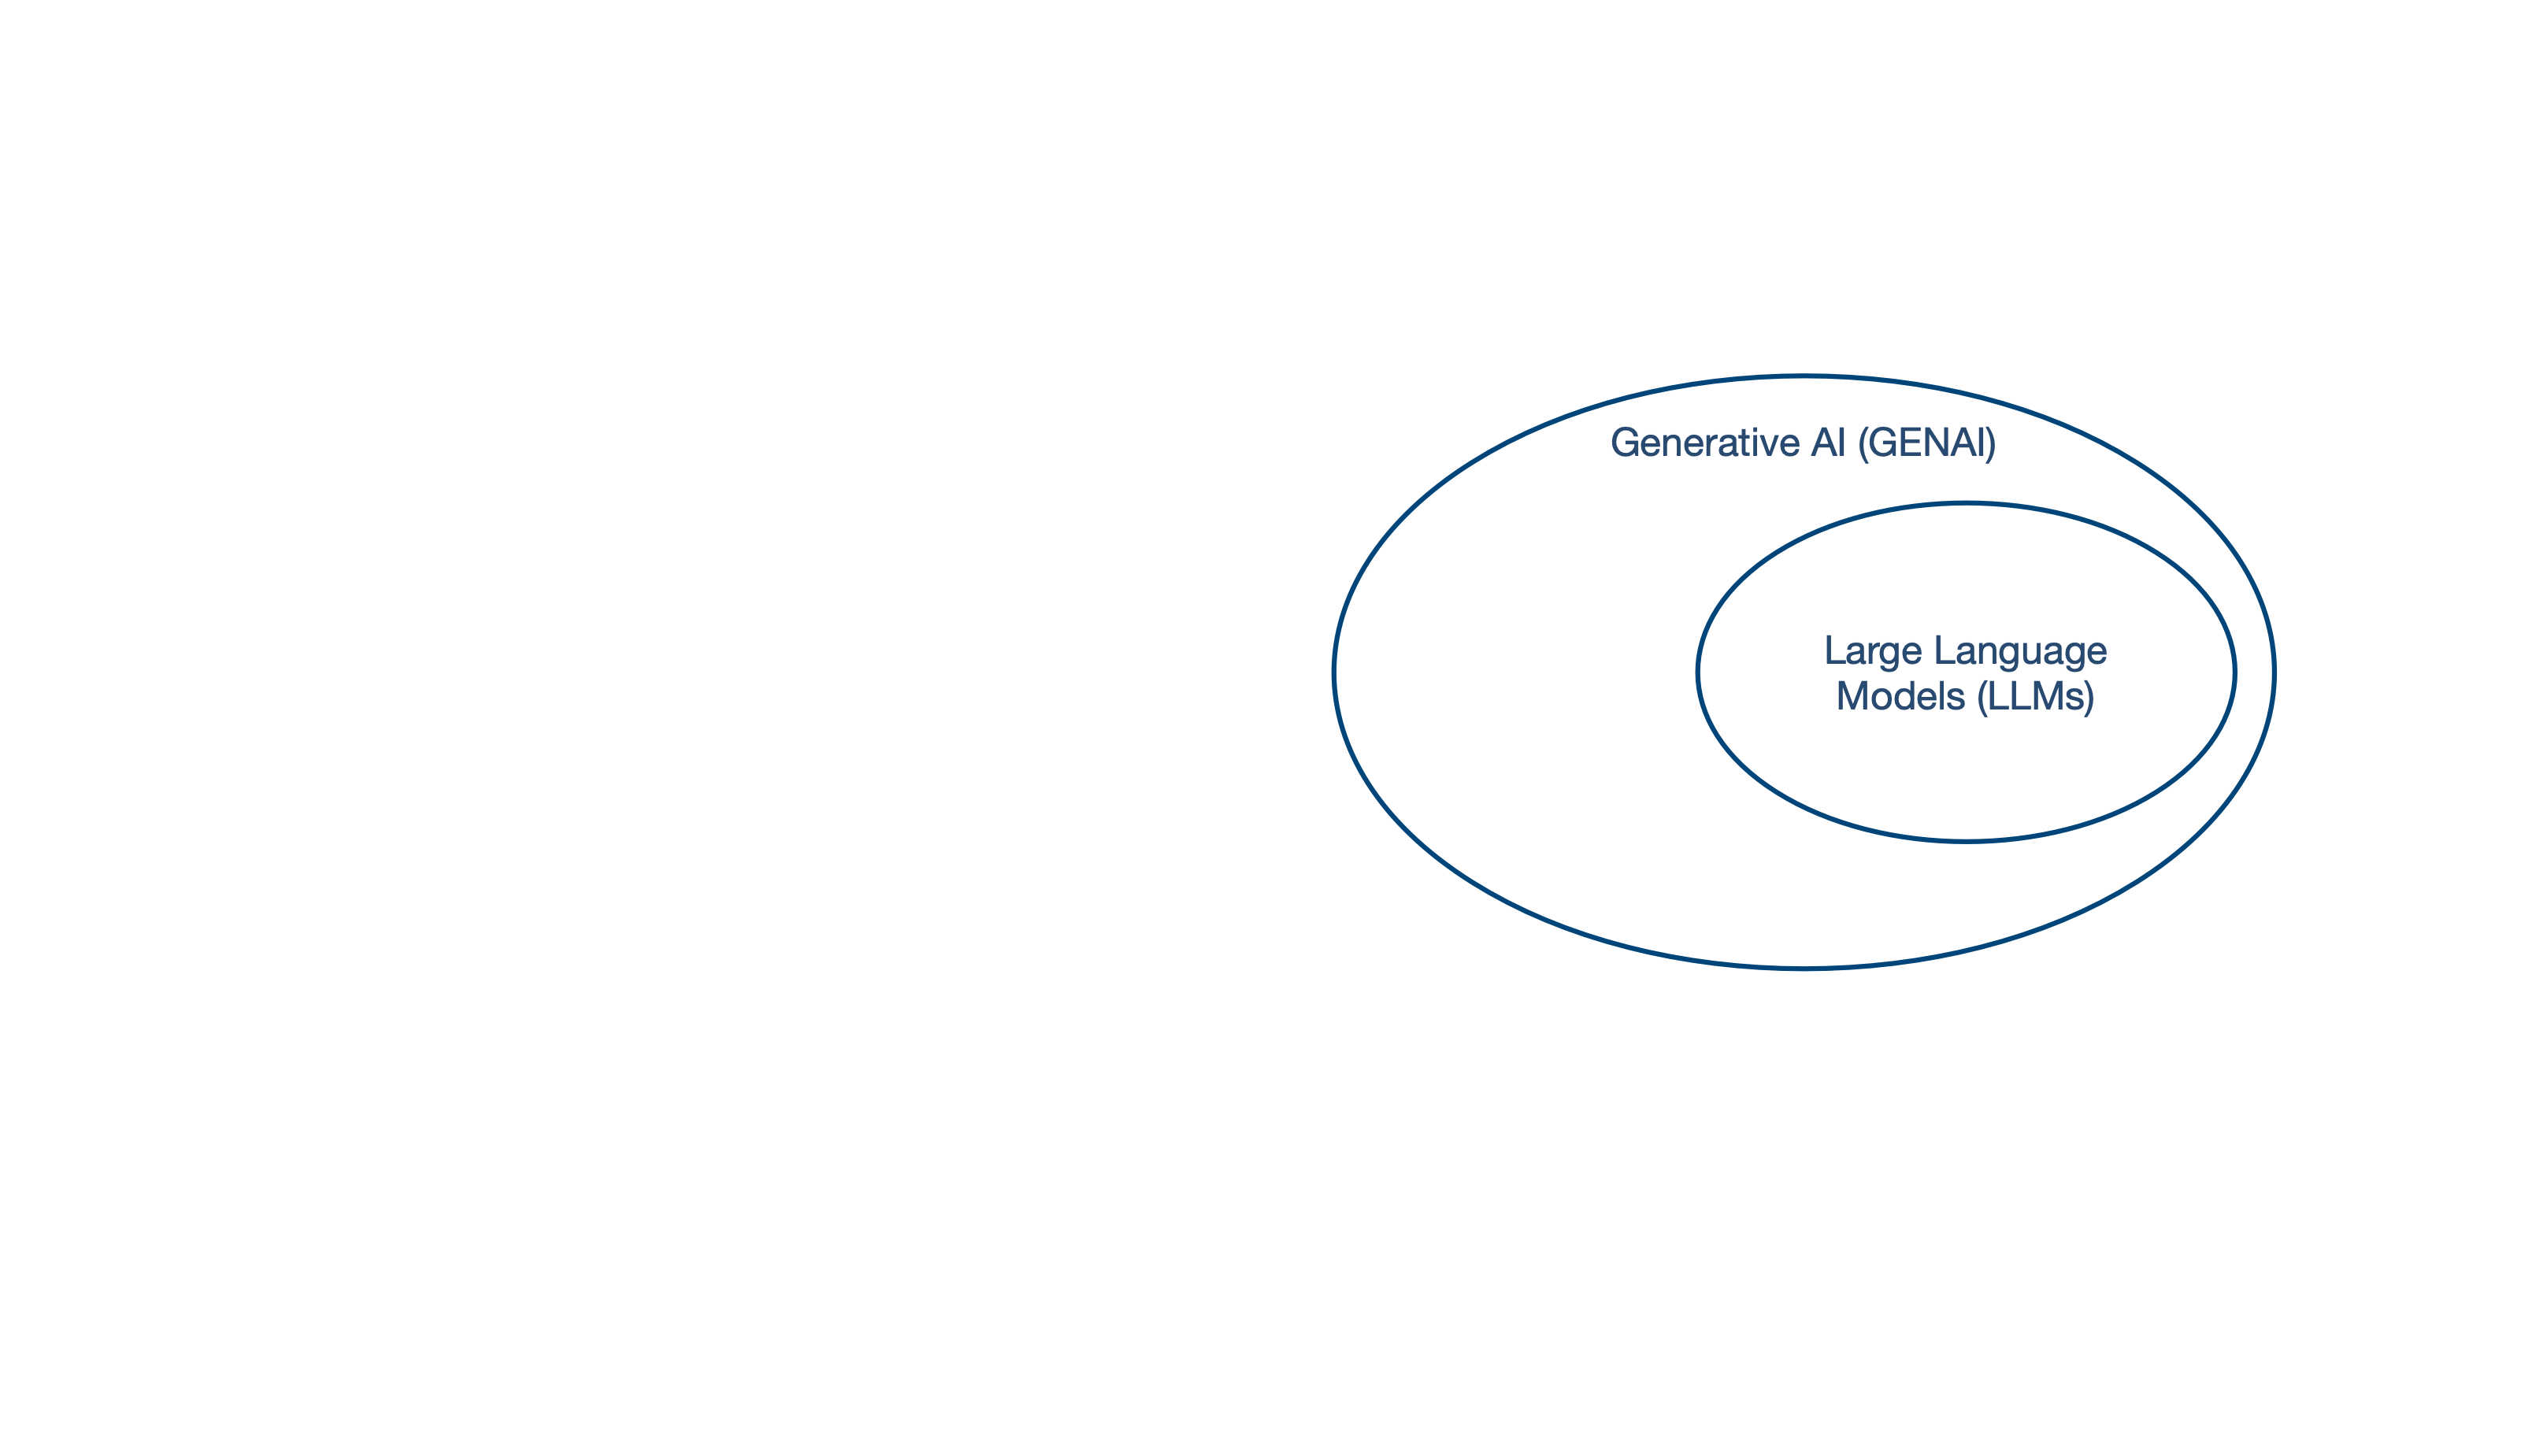
\includegraphics[width=\textwidth]{2.png}
                \end{minipage}
            \end{figure}
        }
        \only<3|handout:0>{
	    \begin{figure}[ht]
                \begin{minipage}[b]{0.95\linewidth}
                    \centering
                    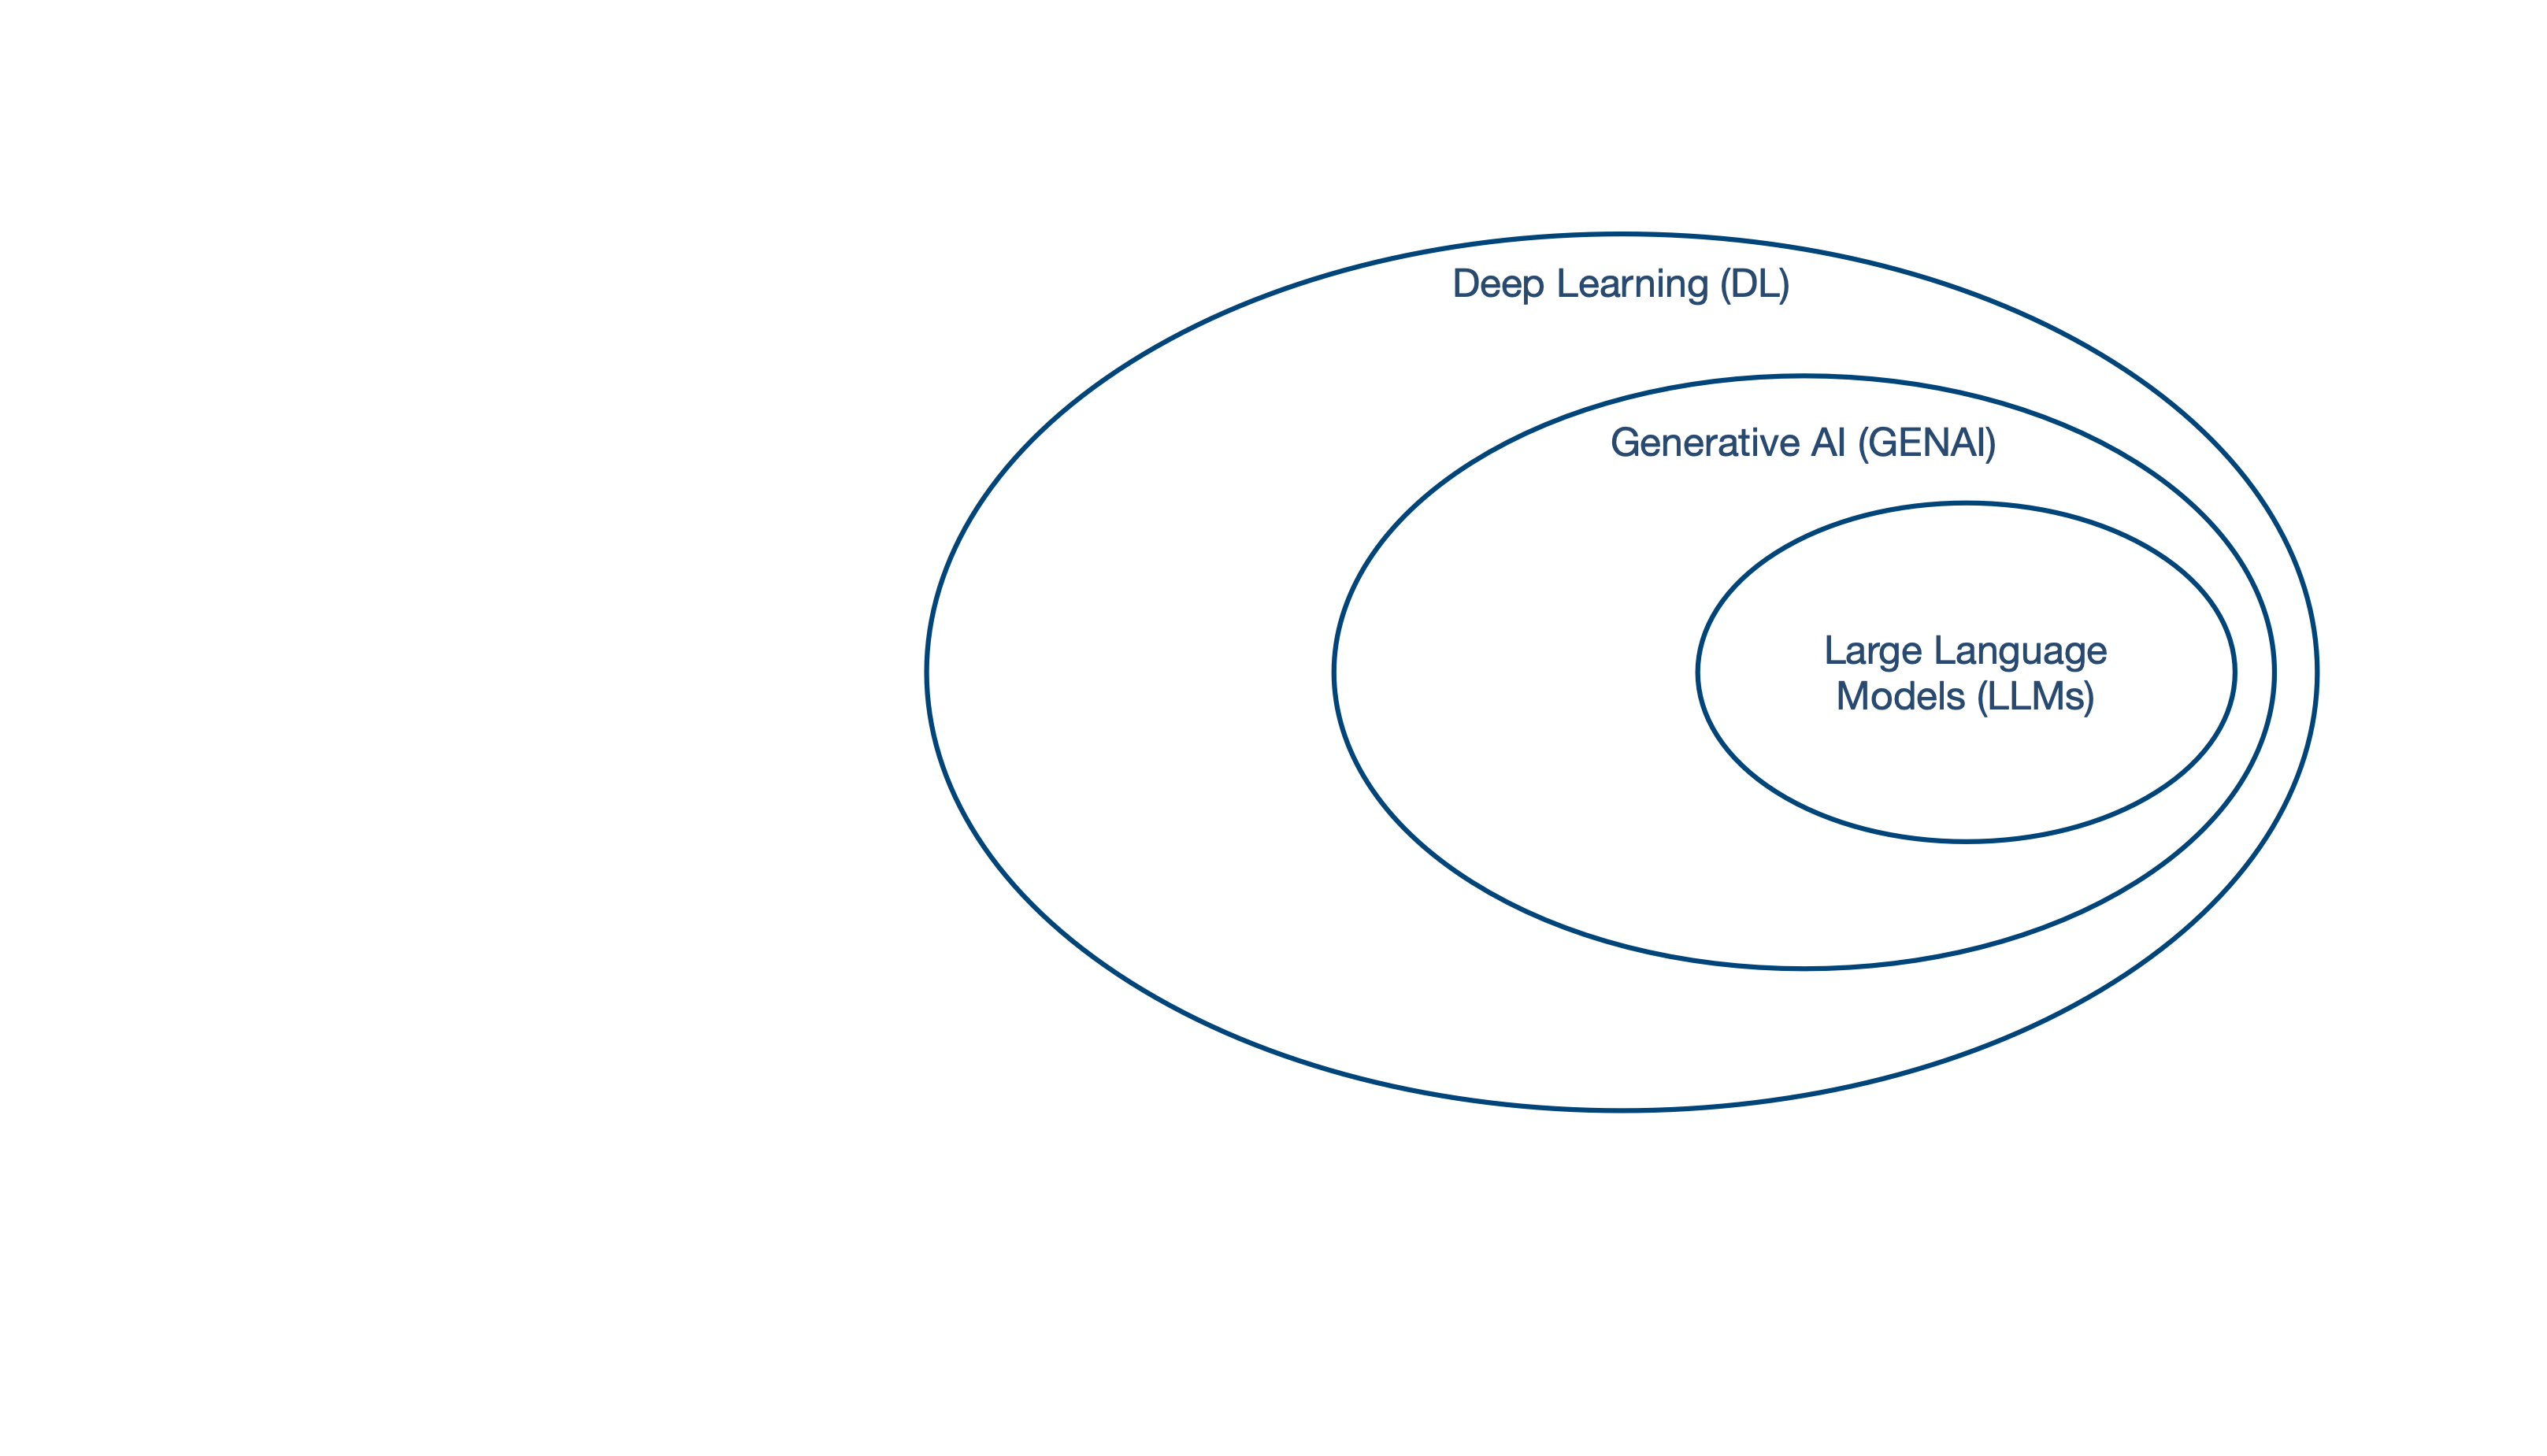
\includegraphics[width=\textwidth]{3.png}
                \end{minipage}
            \end{figure}
        }
        \only<4|handout:0>{
	    \begin{figure}[ht]
                \begin{minipage}[b]{0.95\linewidth}
                    \centering
                    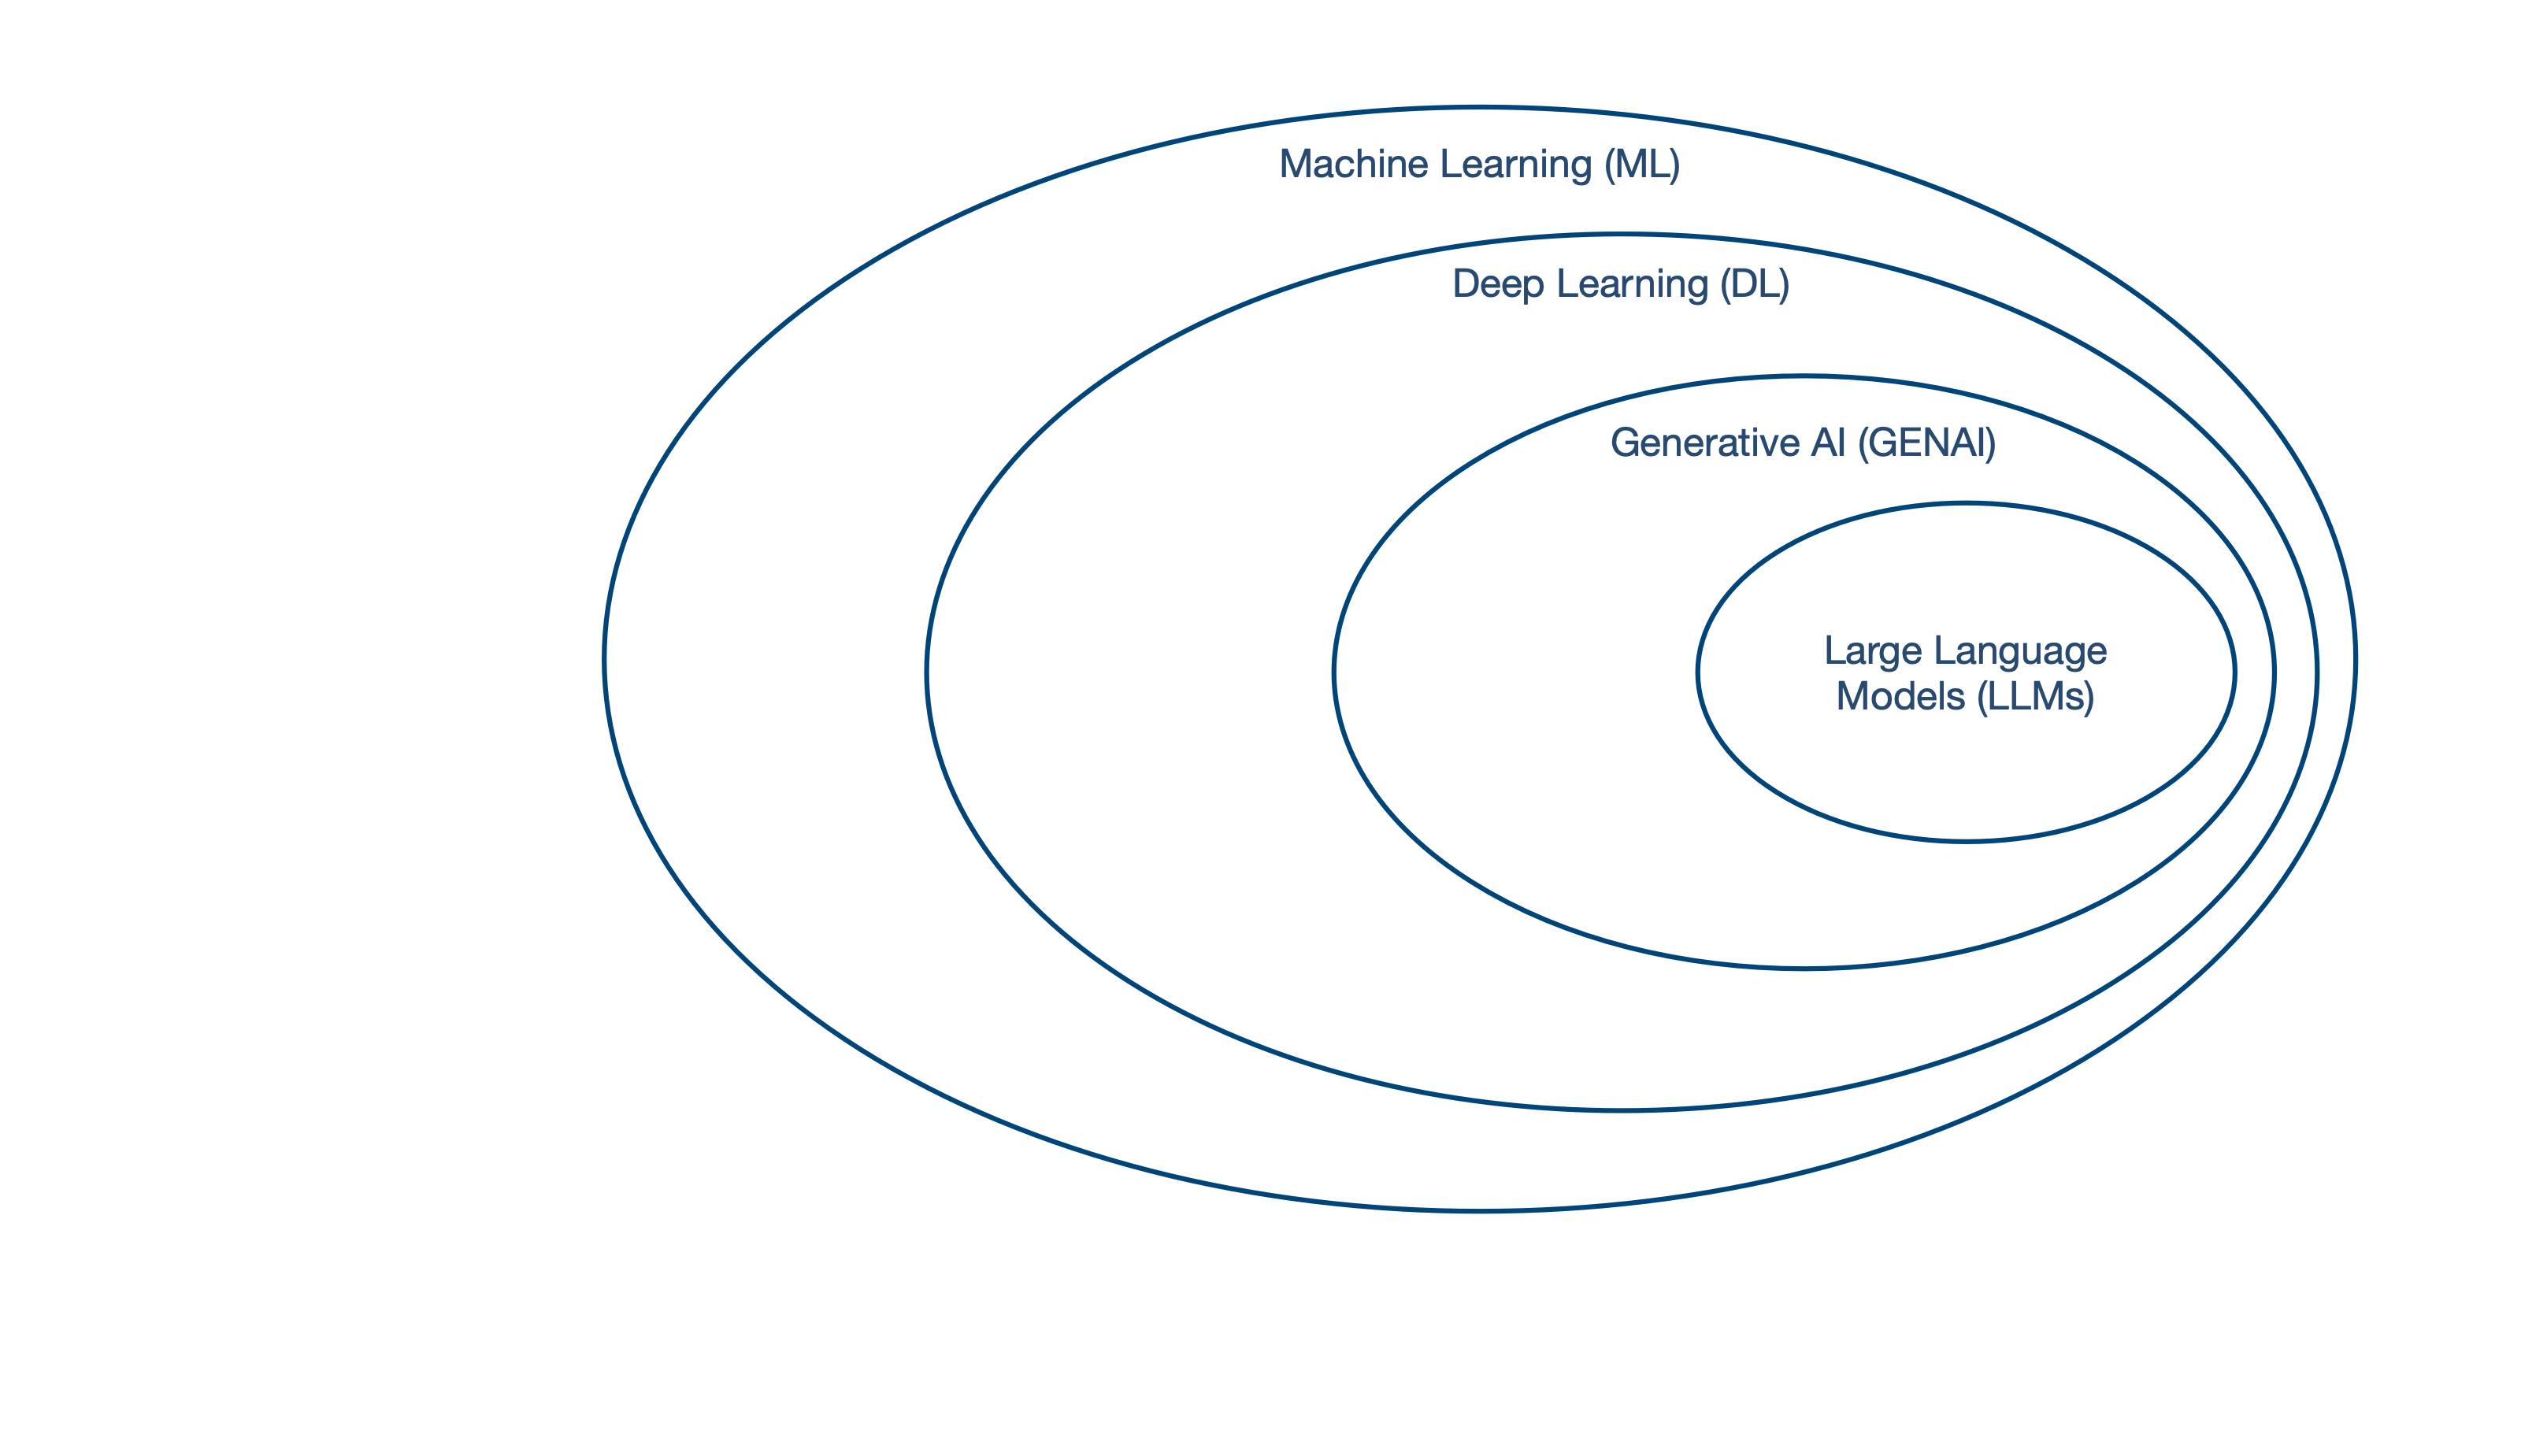
\includegraphics[width=\textwidth]{4.png}
                \end{minipage}
            \end{figure}
        }
        \only<5|handout:0>{
	    \begin{figure}[ht]
                \begin{minipage}[b]{0.95\linewidth}
                    \centering
                    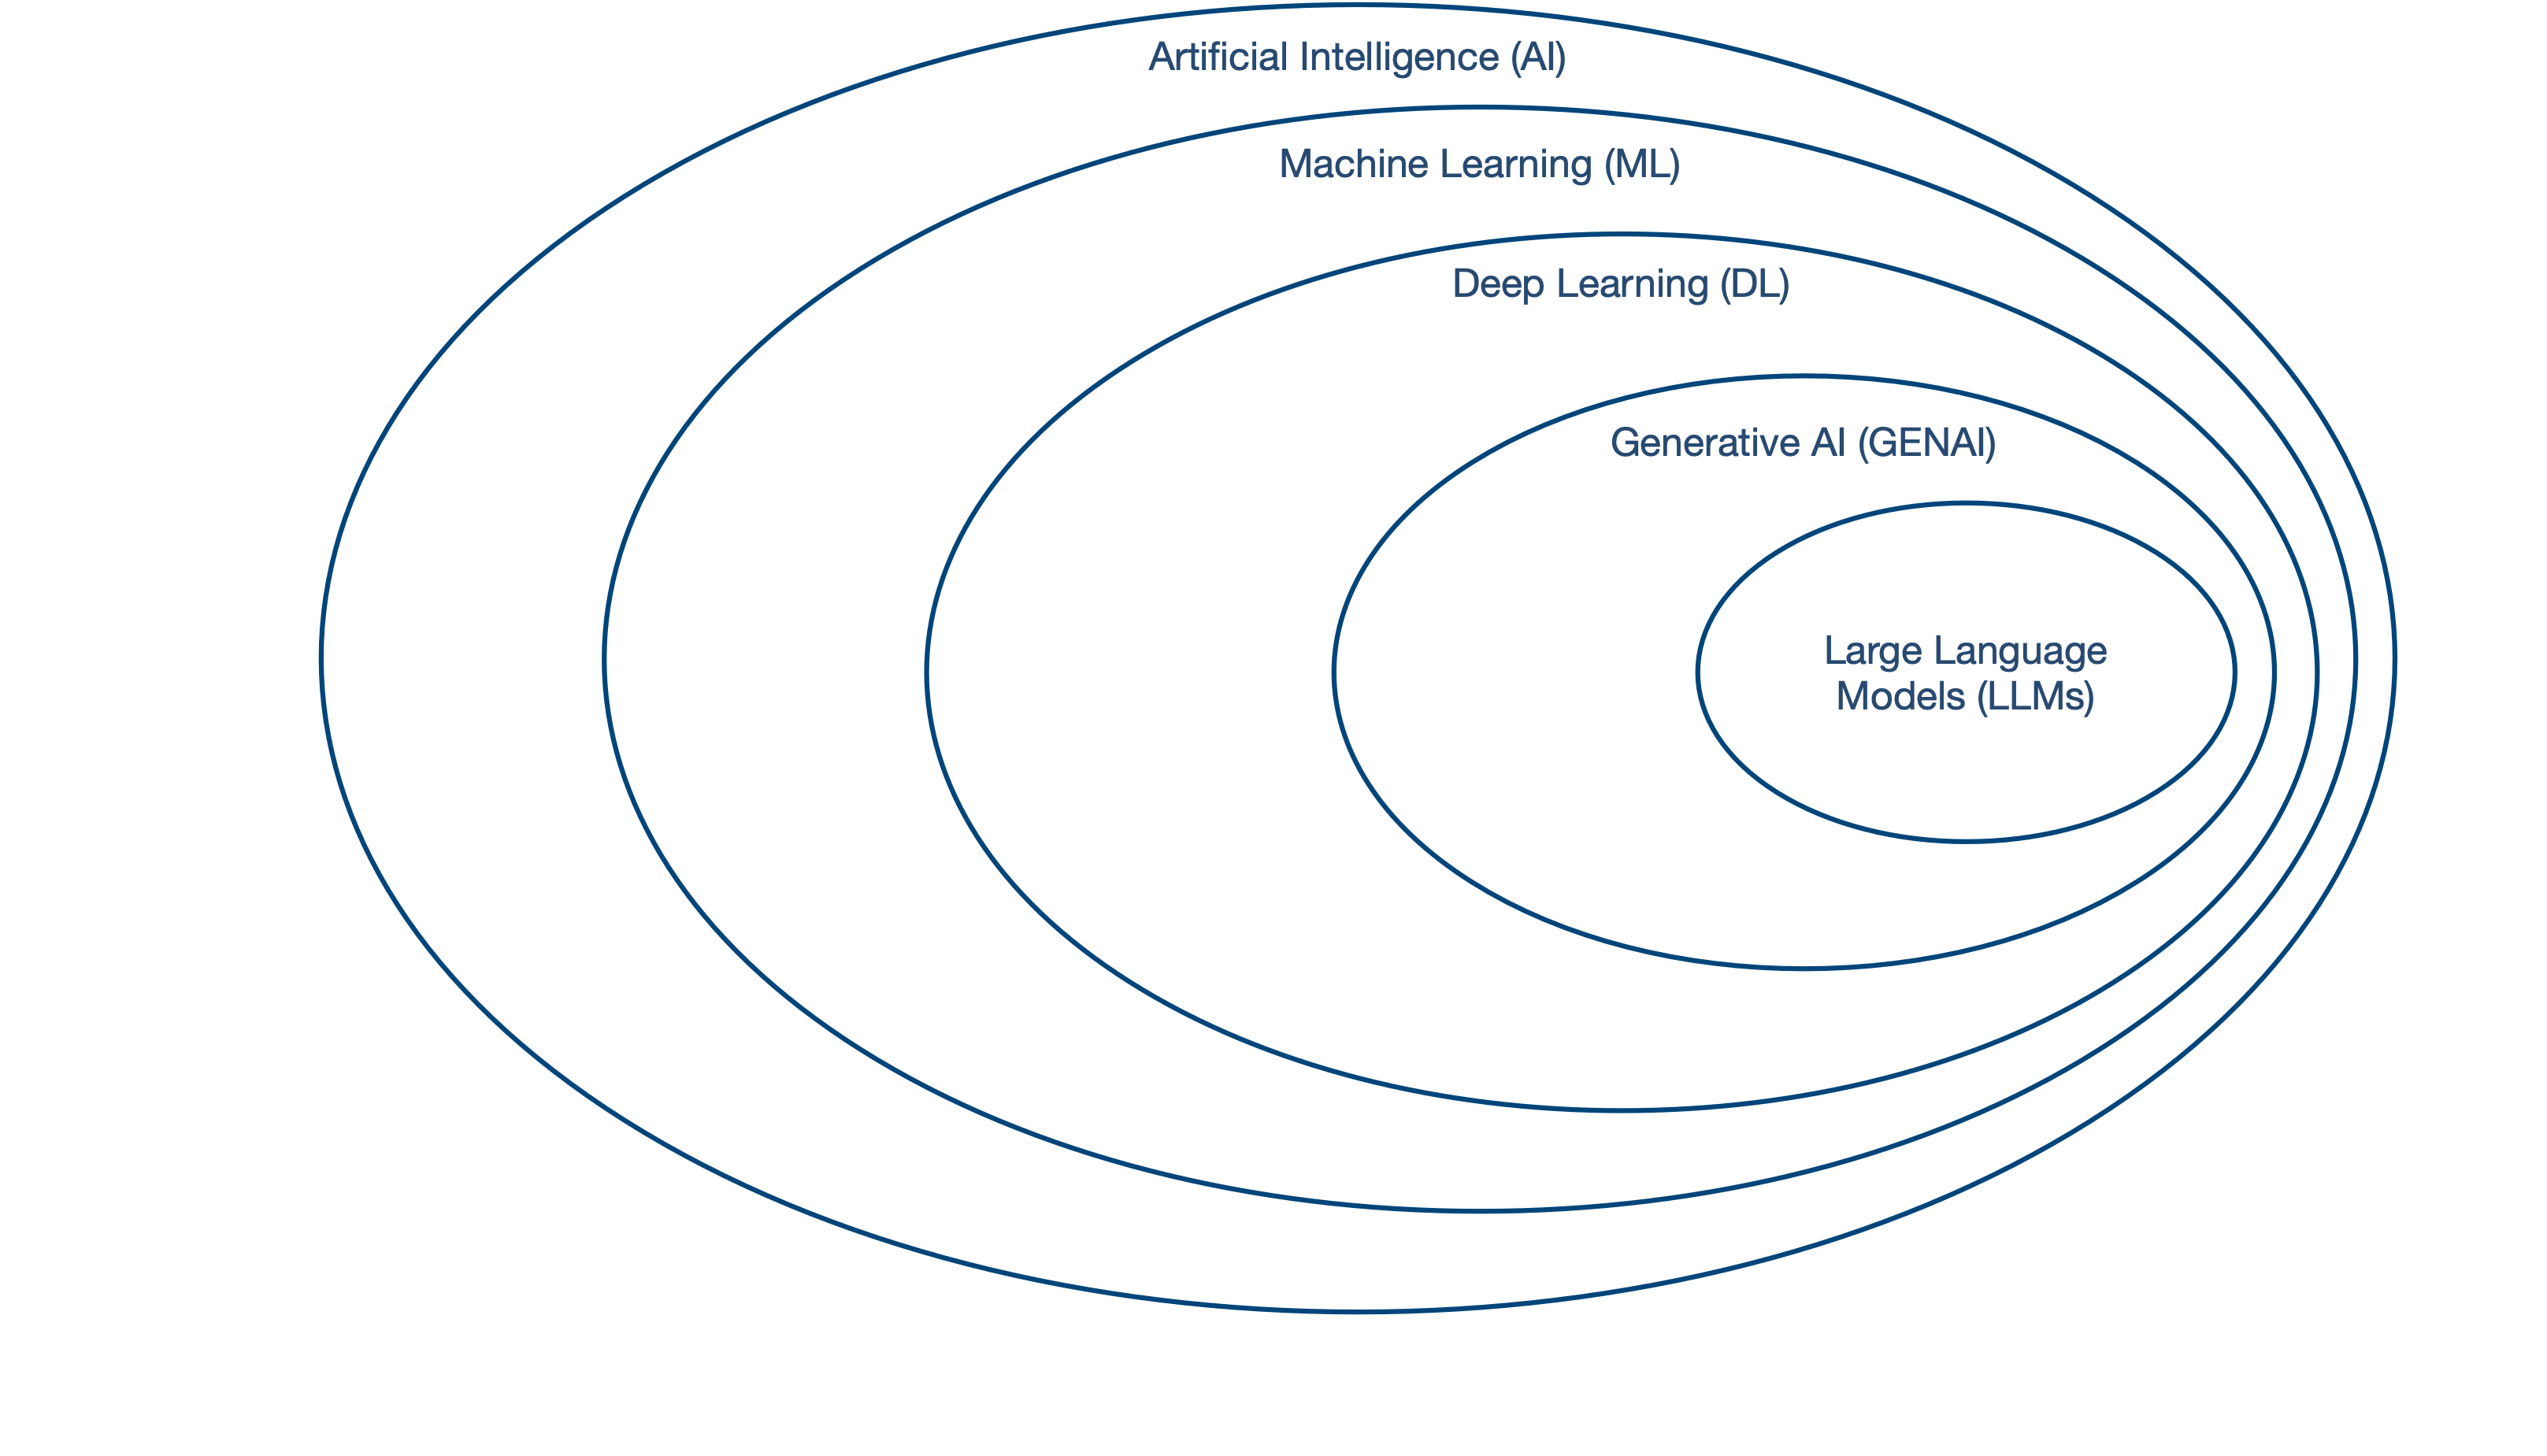
\includegraphics[width=\textwidth]{5.png}
                \end{minipage}
            \end{figure}
        }
        \only<6|handout:0>{
        \begin{figure}[ht]
            \begin{minipage}[b]{0.95\linewidth}
                \centering
                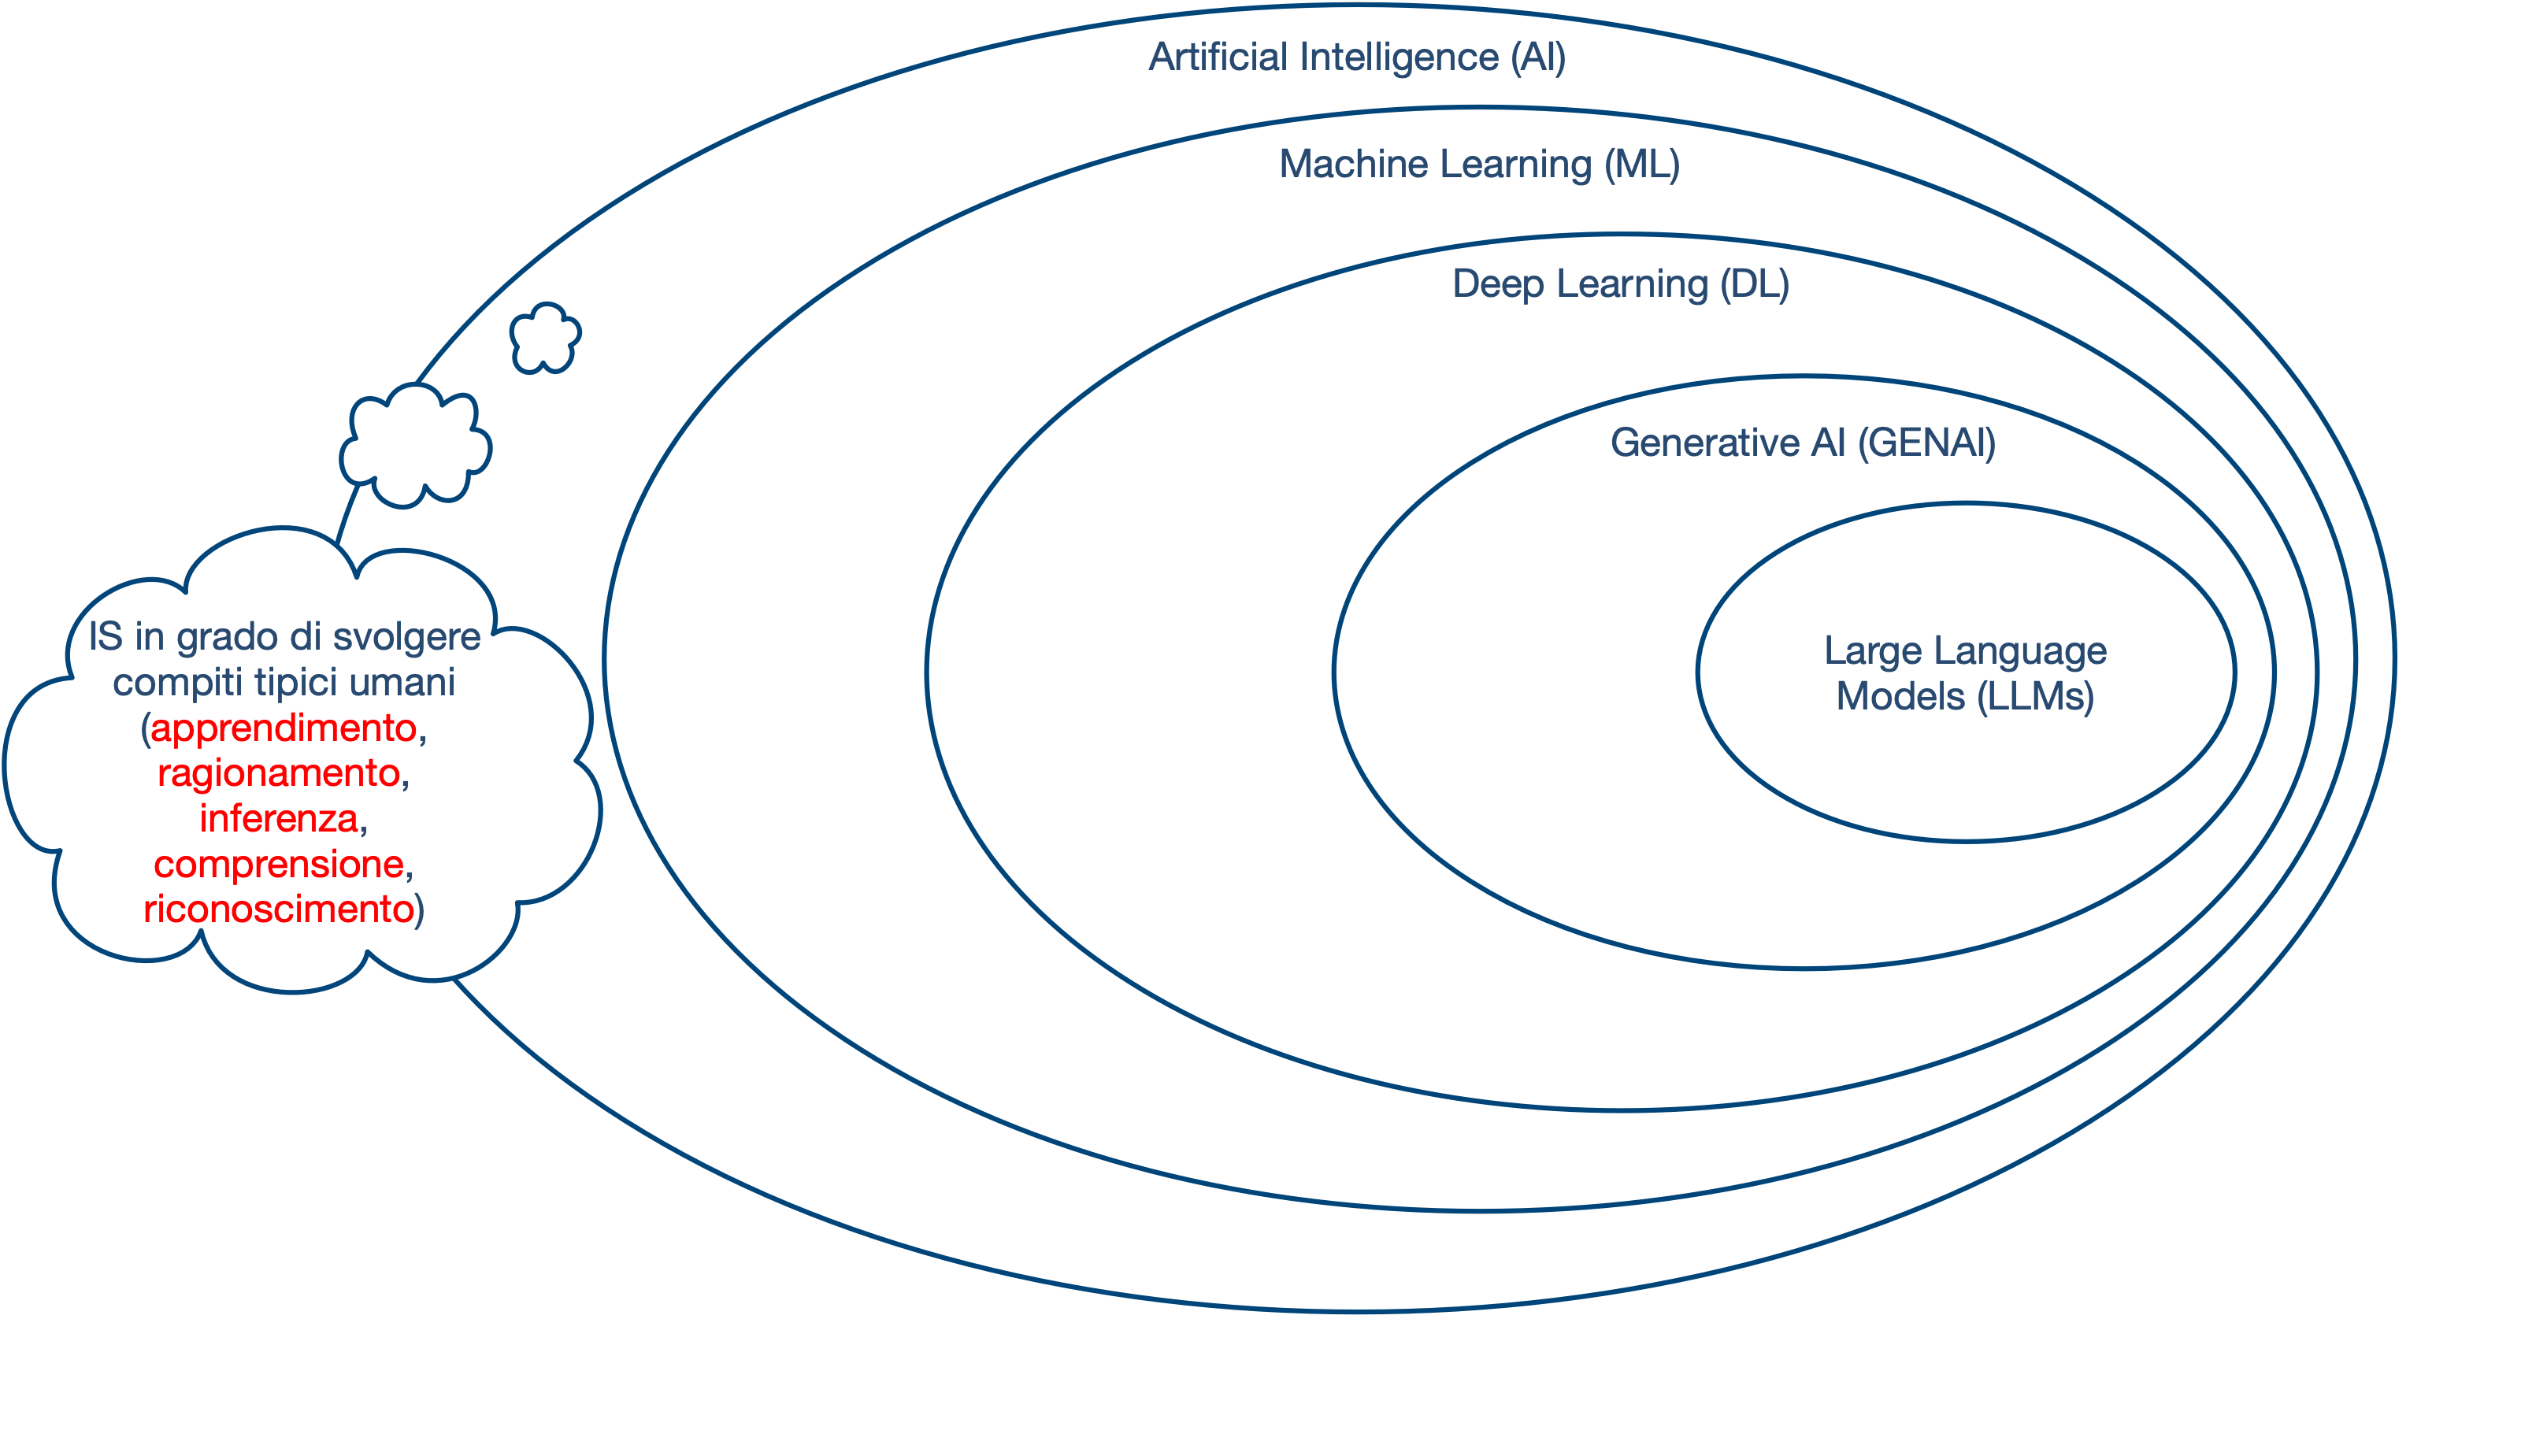
\includegraphics[width=\textwidth]{6.png}
            \end{minipage}
        \end{figure}
        }
        \only<7|handout:0>{
        \begin{figure}[ht]
            \begin{minipage}[b]{0.95\linewidth}
                \centering
                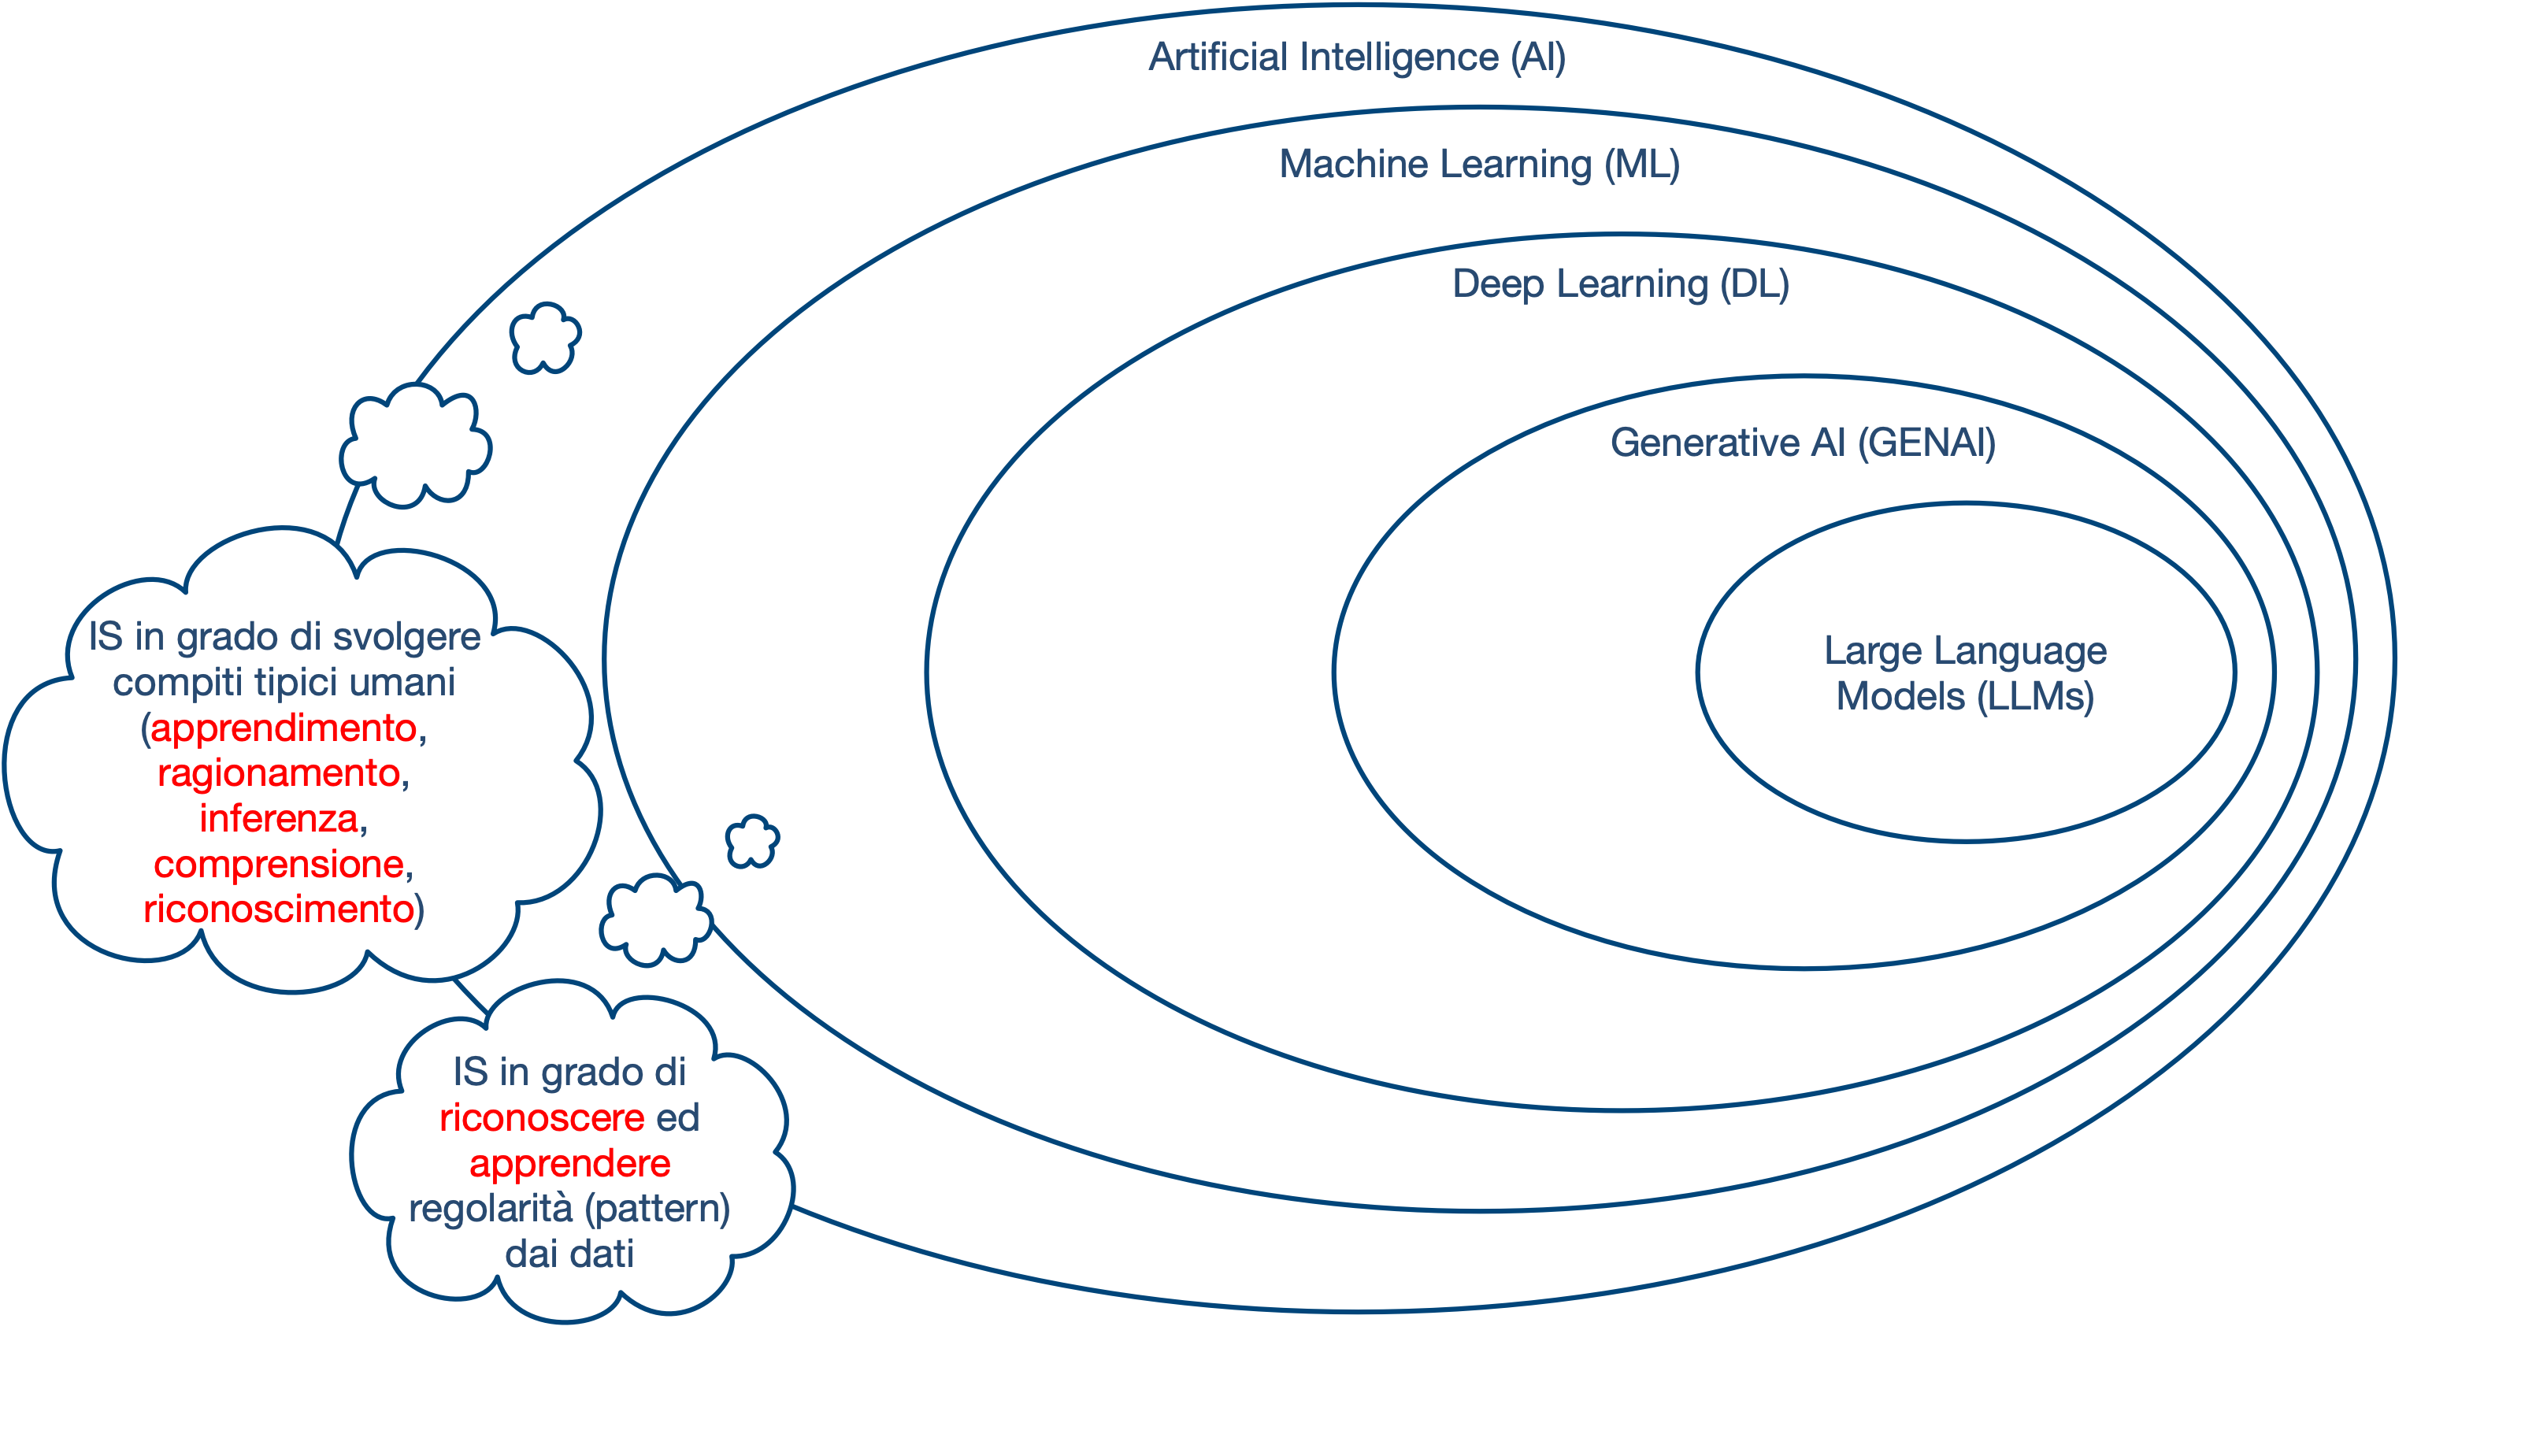
\includegraphics[width=\textwidth]{7.png}
            \end{minipage}
        \end{figure}
        }
        \only<8|handout:0>{
        \begin{figure}[ht]
            \begin{minipage}[b]{0.95\linewidth}
                \centering
                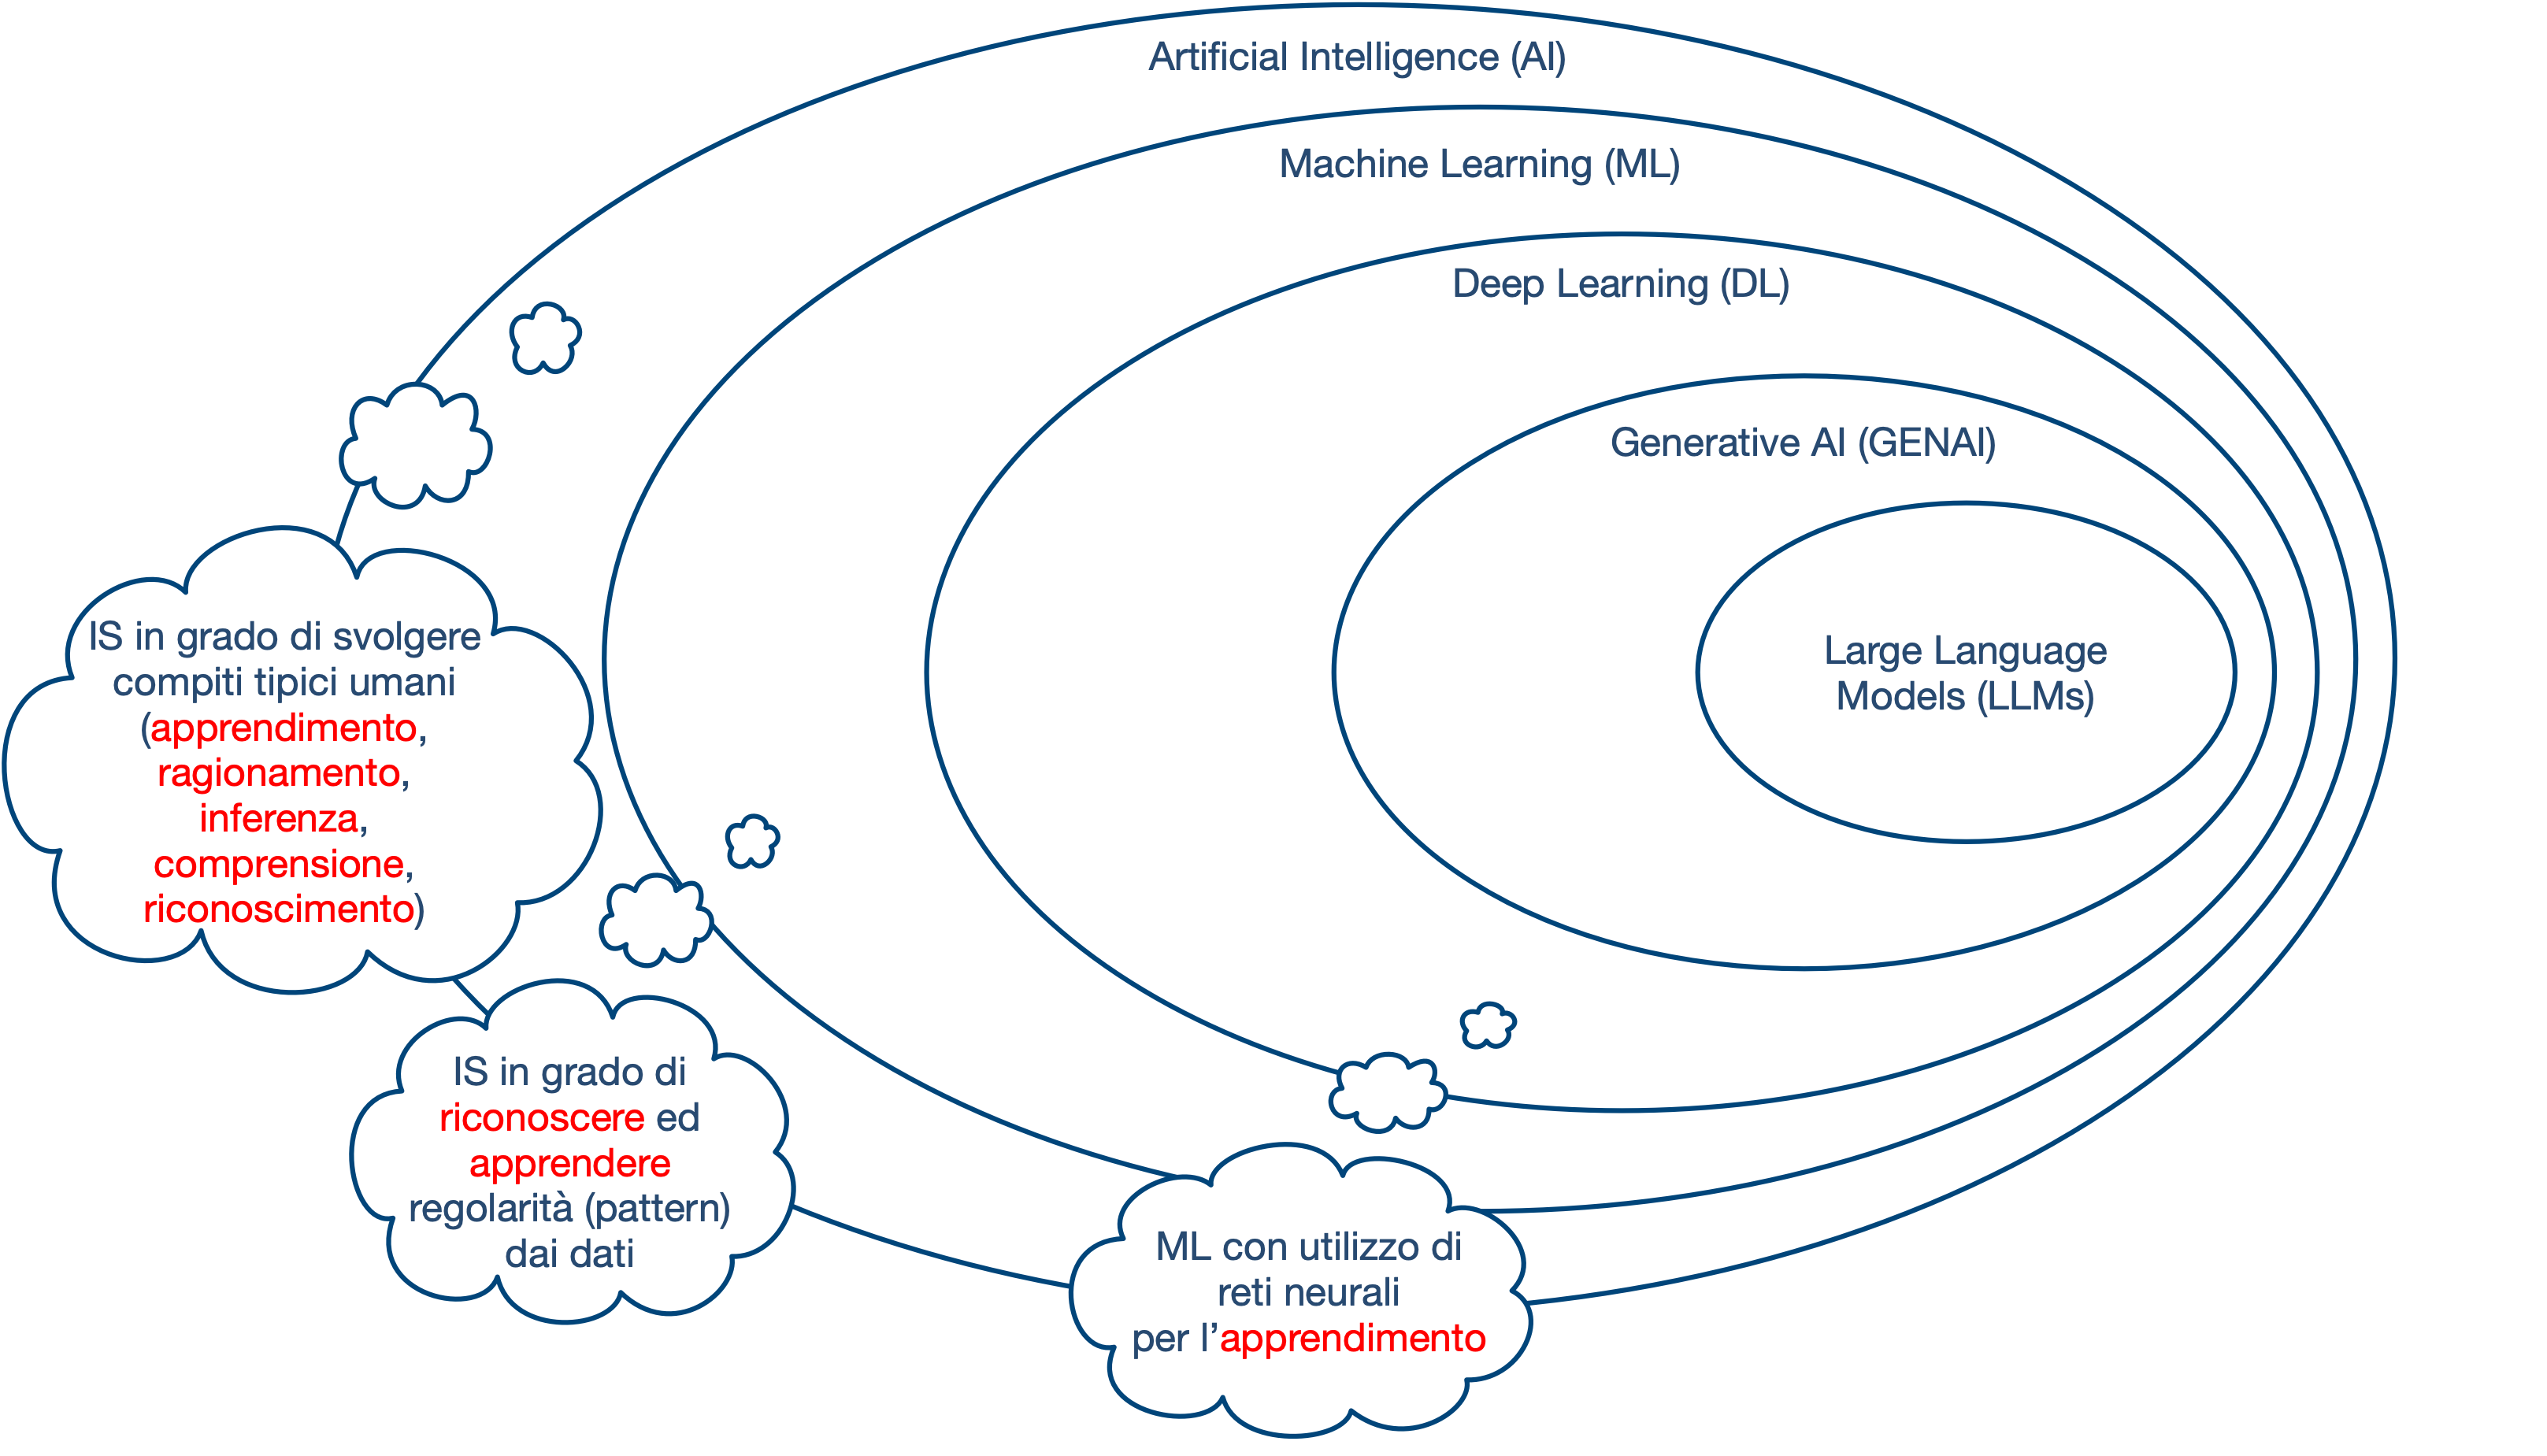
\includegraphics[width=\textwidth]{8.png}
            \end{minipage}
        \end{figure}
        }
        \only<9|handout:0>{
        \begin{figure}[ht]
            \begin{minipage}[b]{0.95\linewidth}
                \centering
                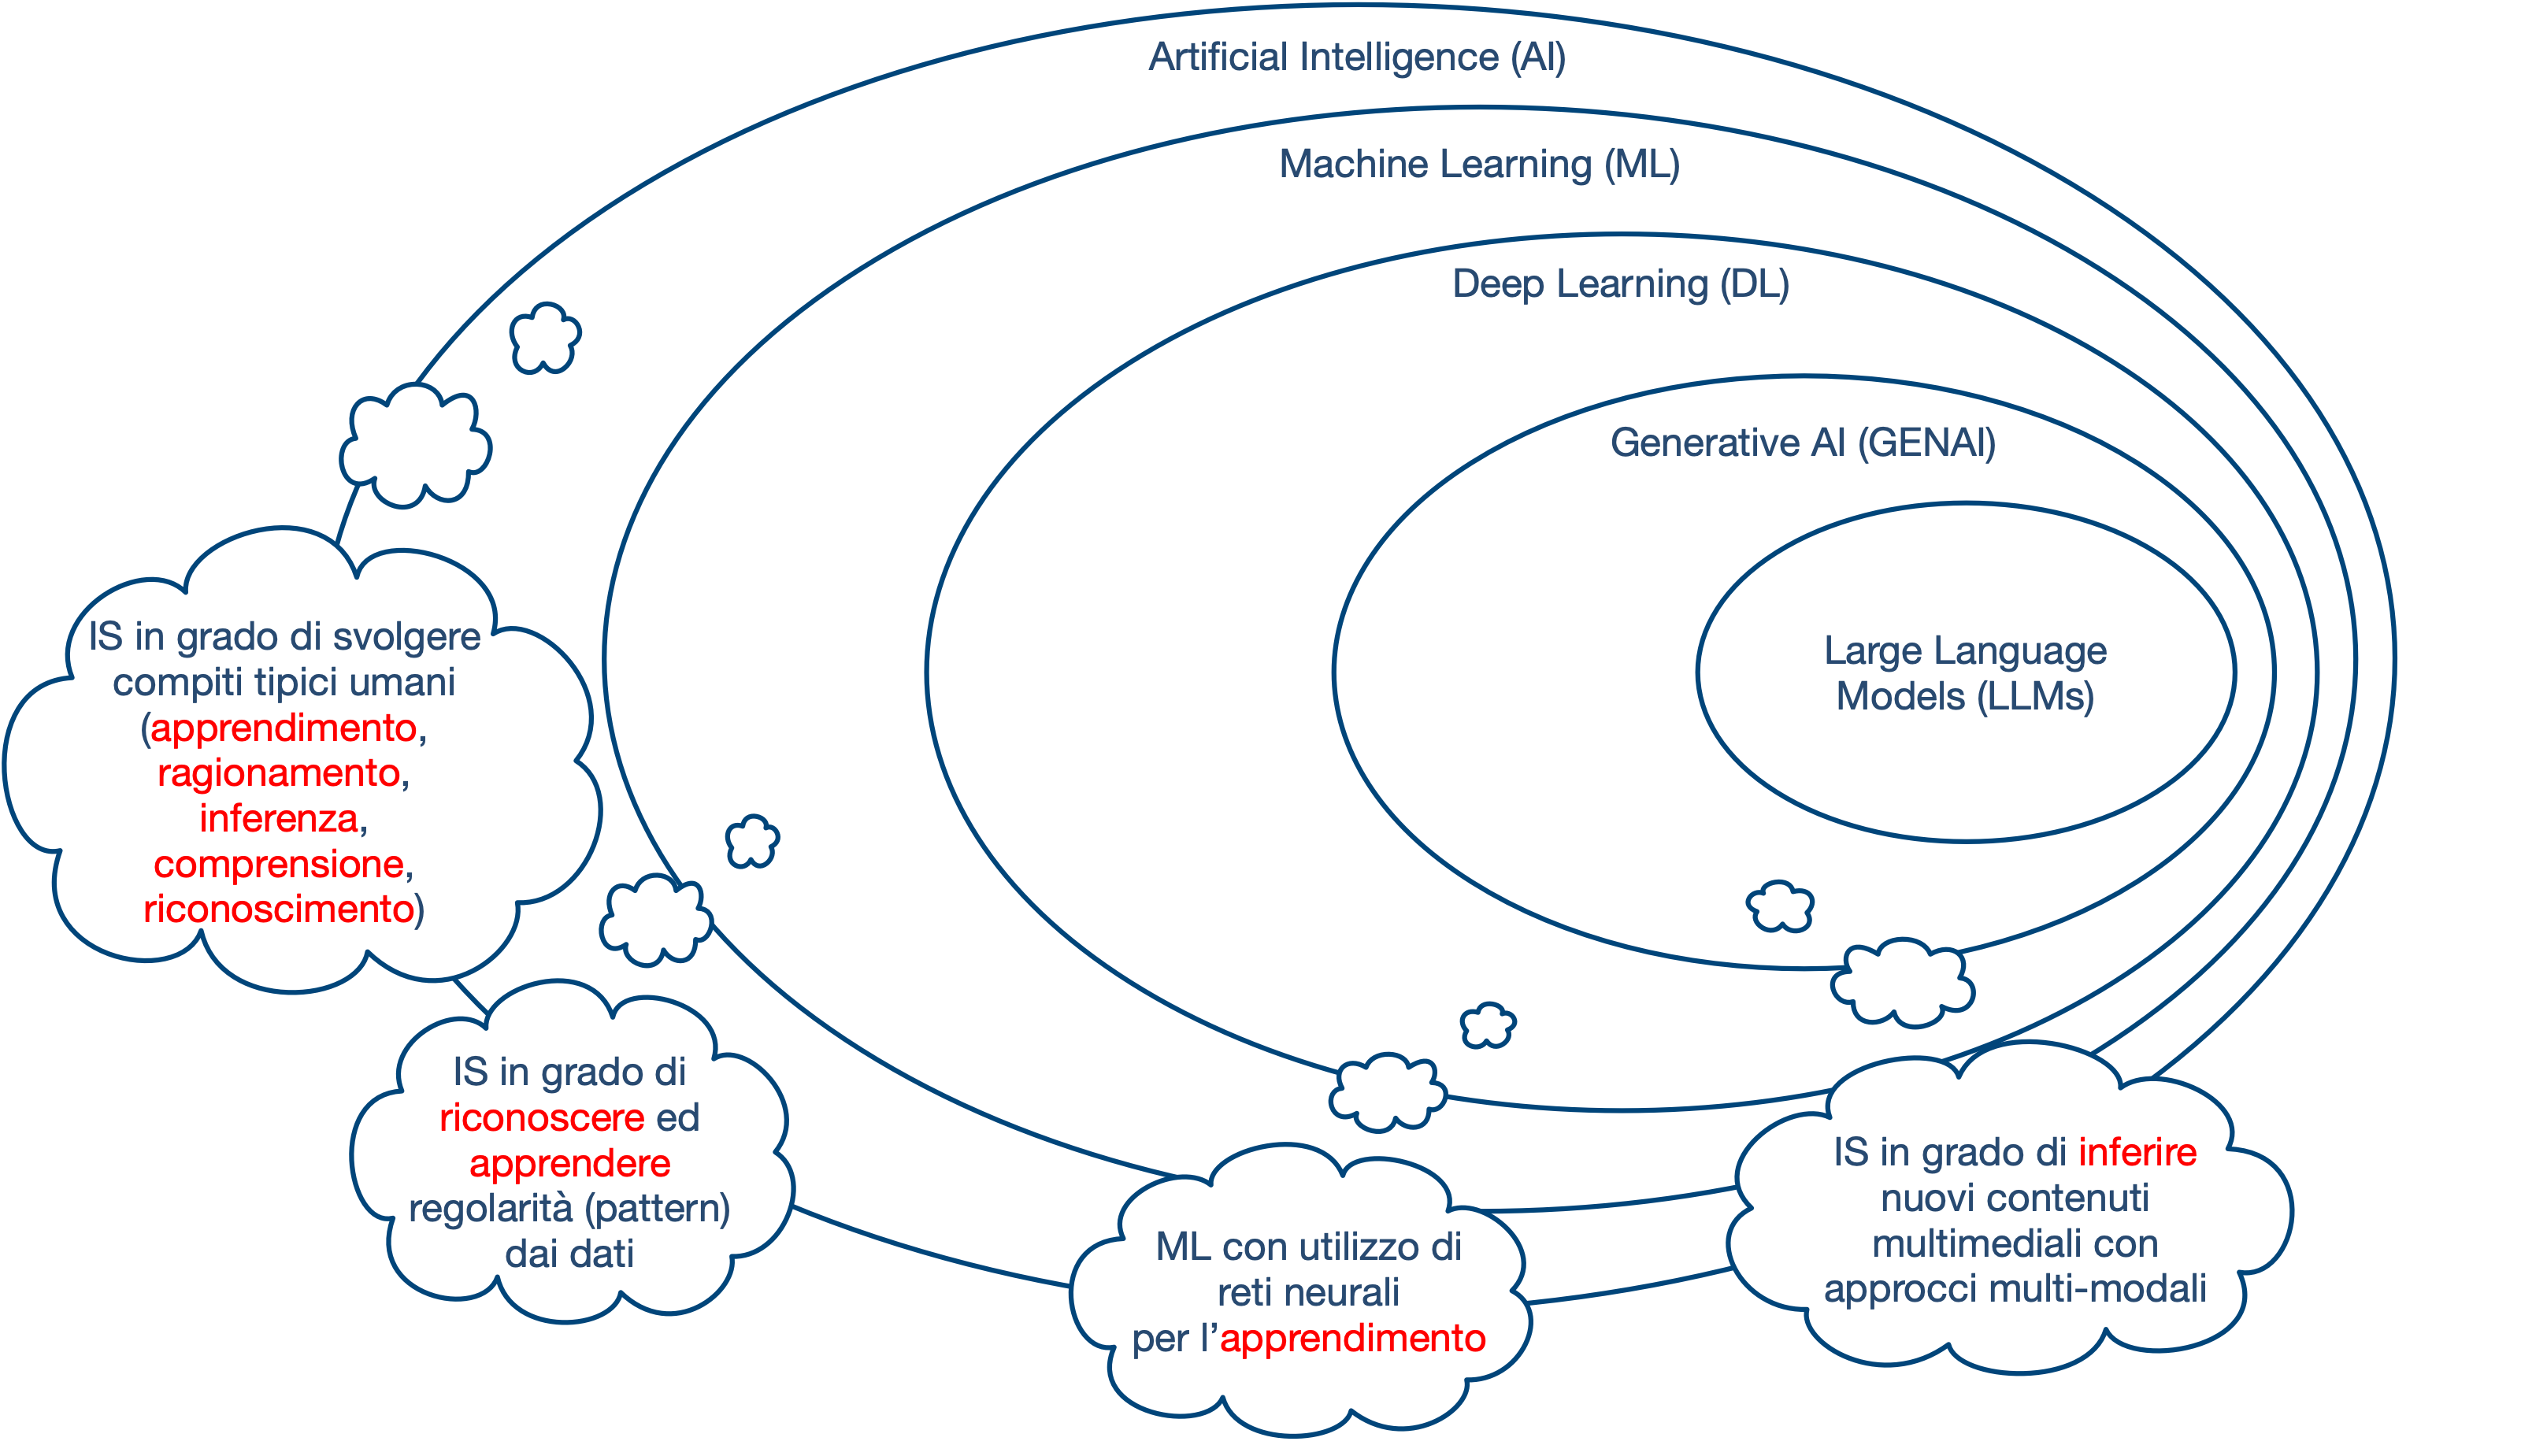
\includegraphics[width=\textwidth]{9.png}
            \end{minipage}
        \end{figure}
        }
        \only<10|handout:0>{
        \begin{figure}[ht]
            \begin{minipage}[b]{0.95\linewidth}
                \centering
                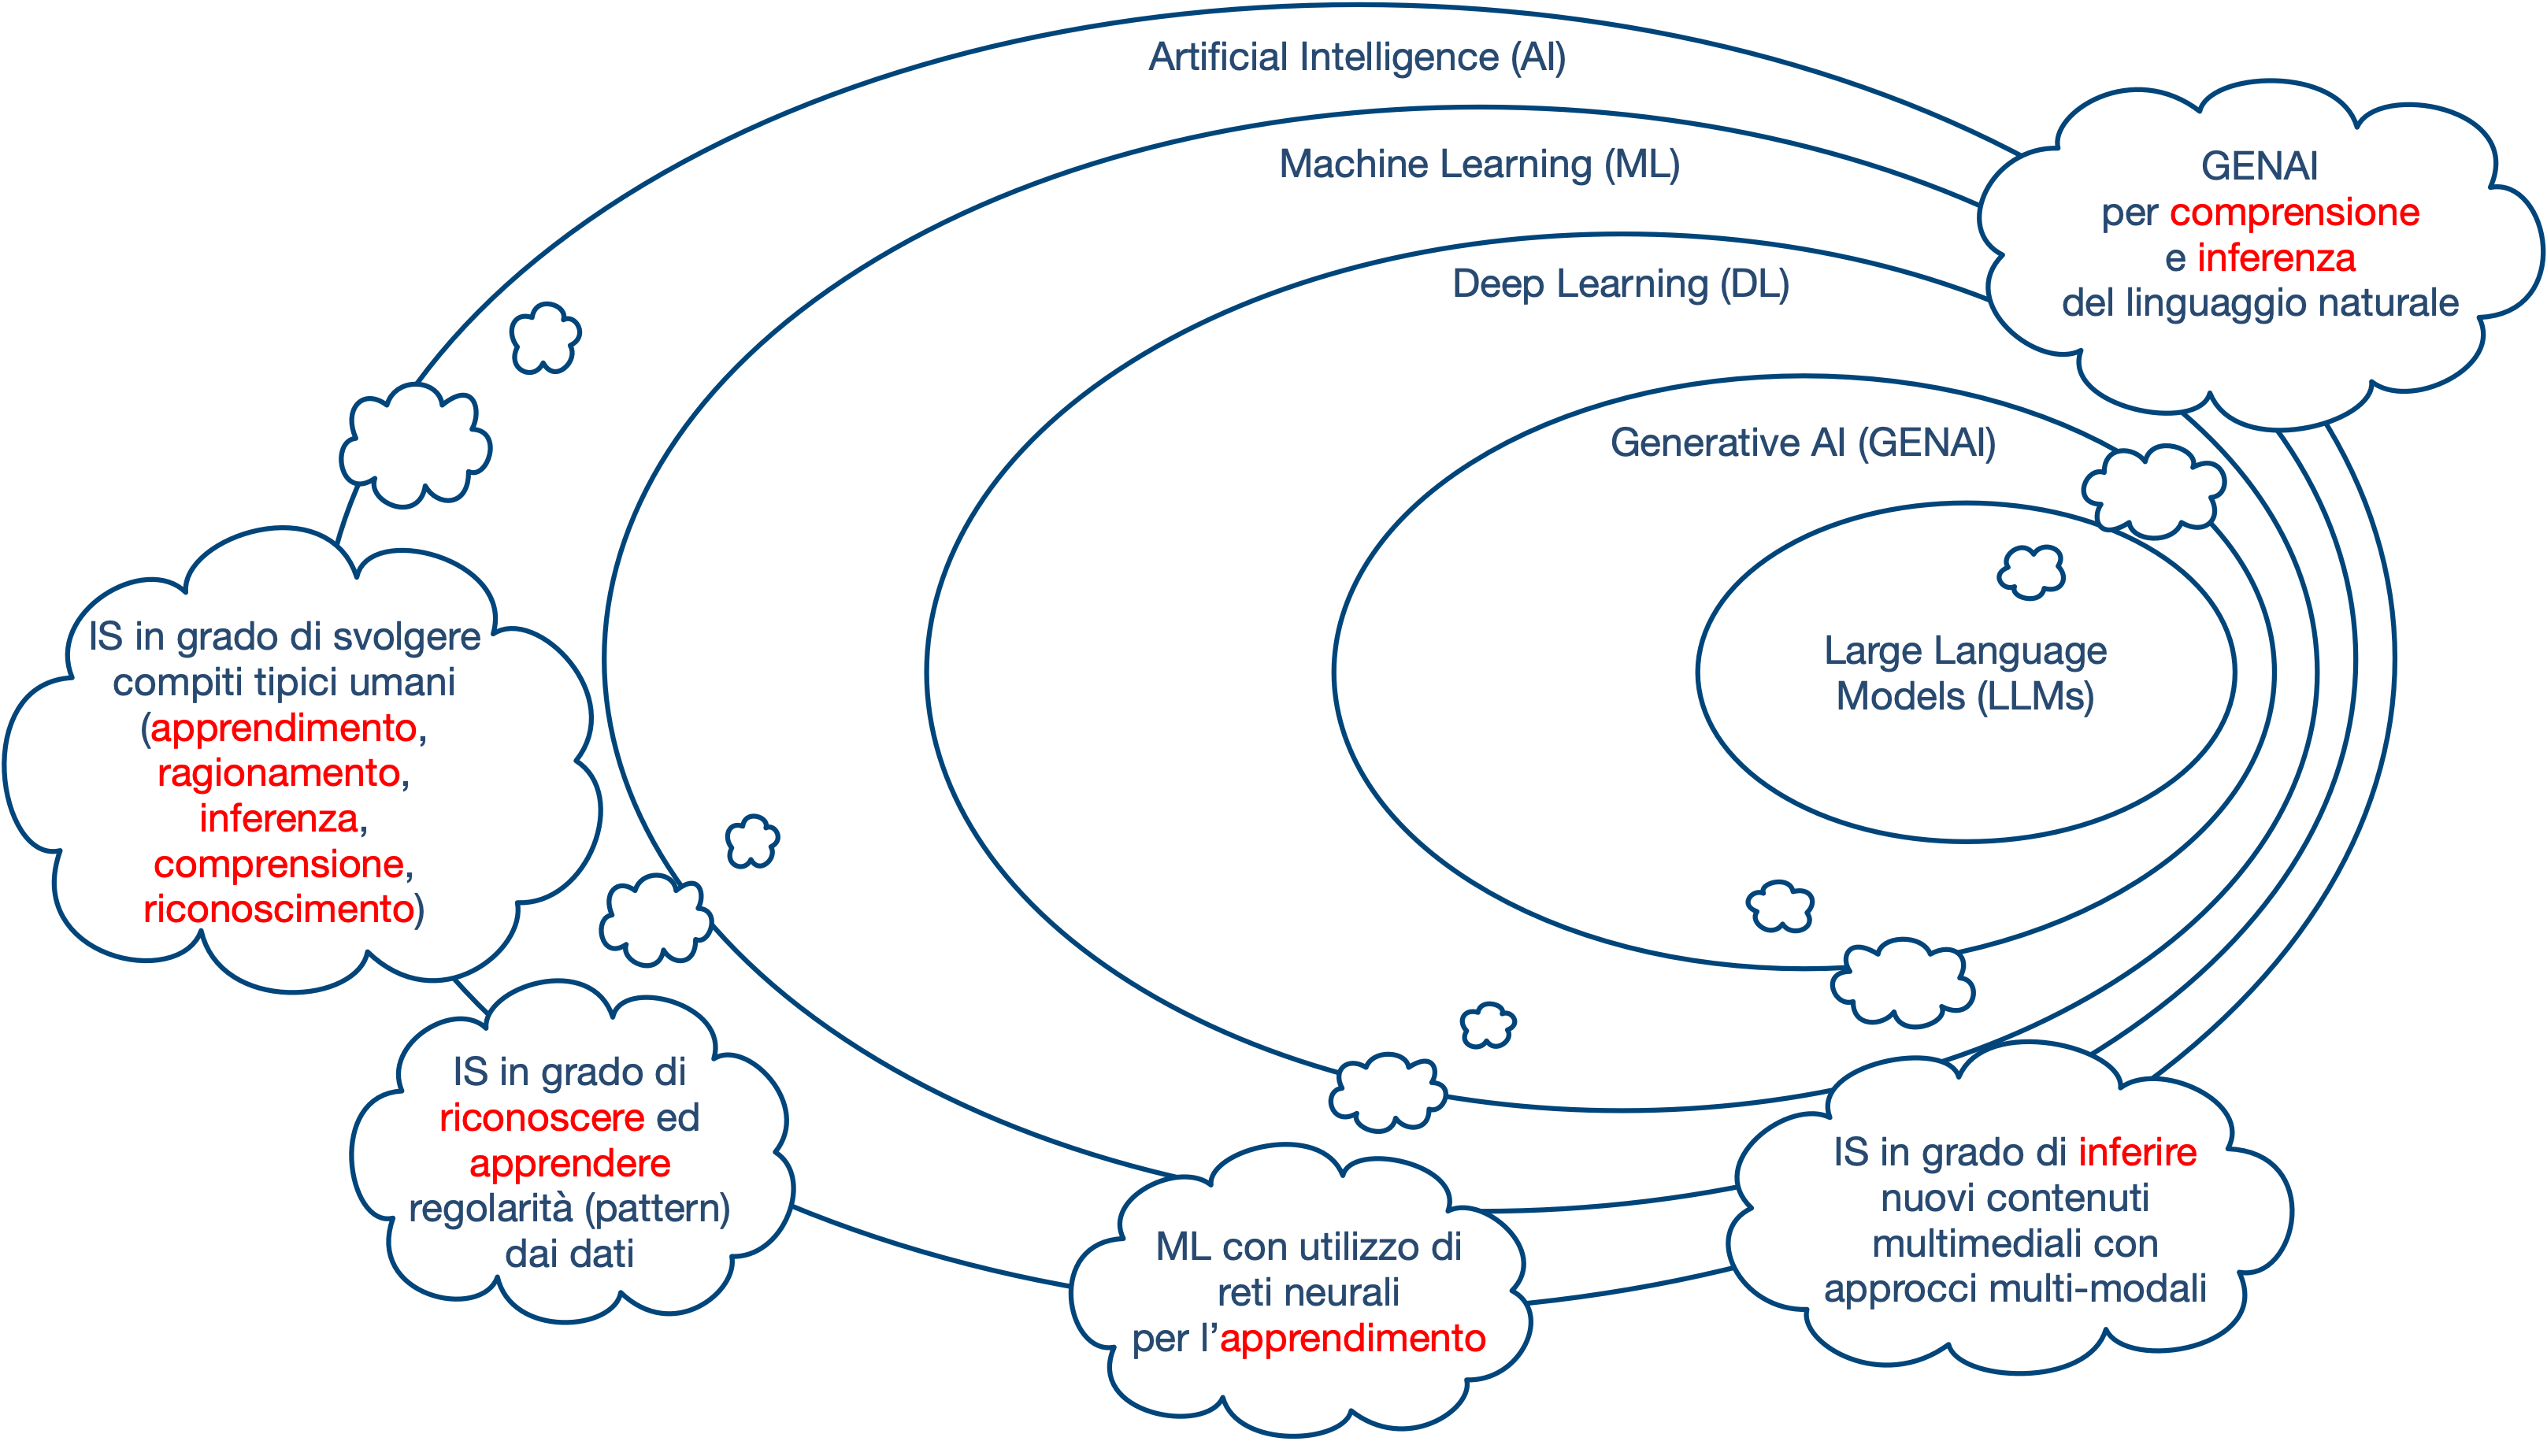
\includegraphics[width=\textwidth]{10.png}
            \end{minipage}
        \end{figure}
        }
        \only<11>{
        \begin{figure}[ht]
            \begin{minipage}[b]{0.95\linewidth}
                \centering
                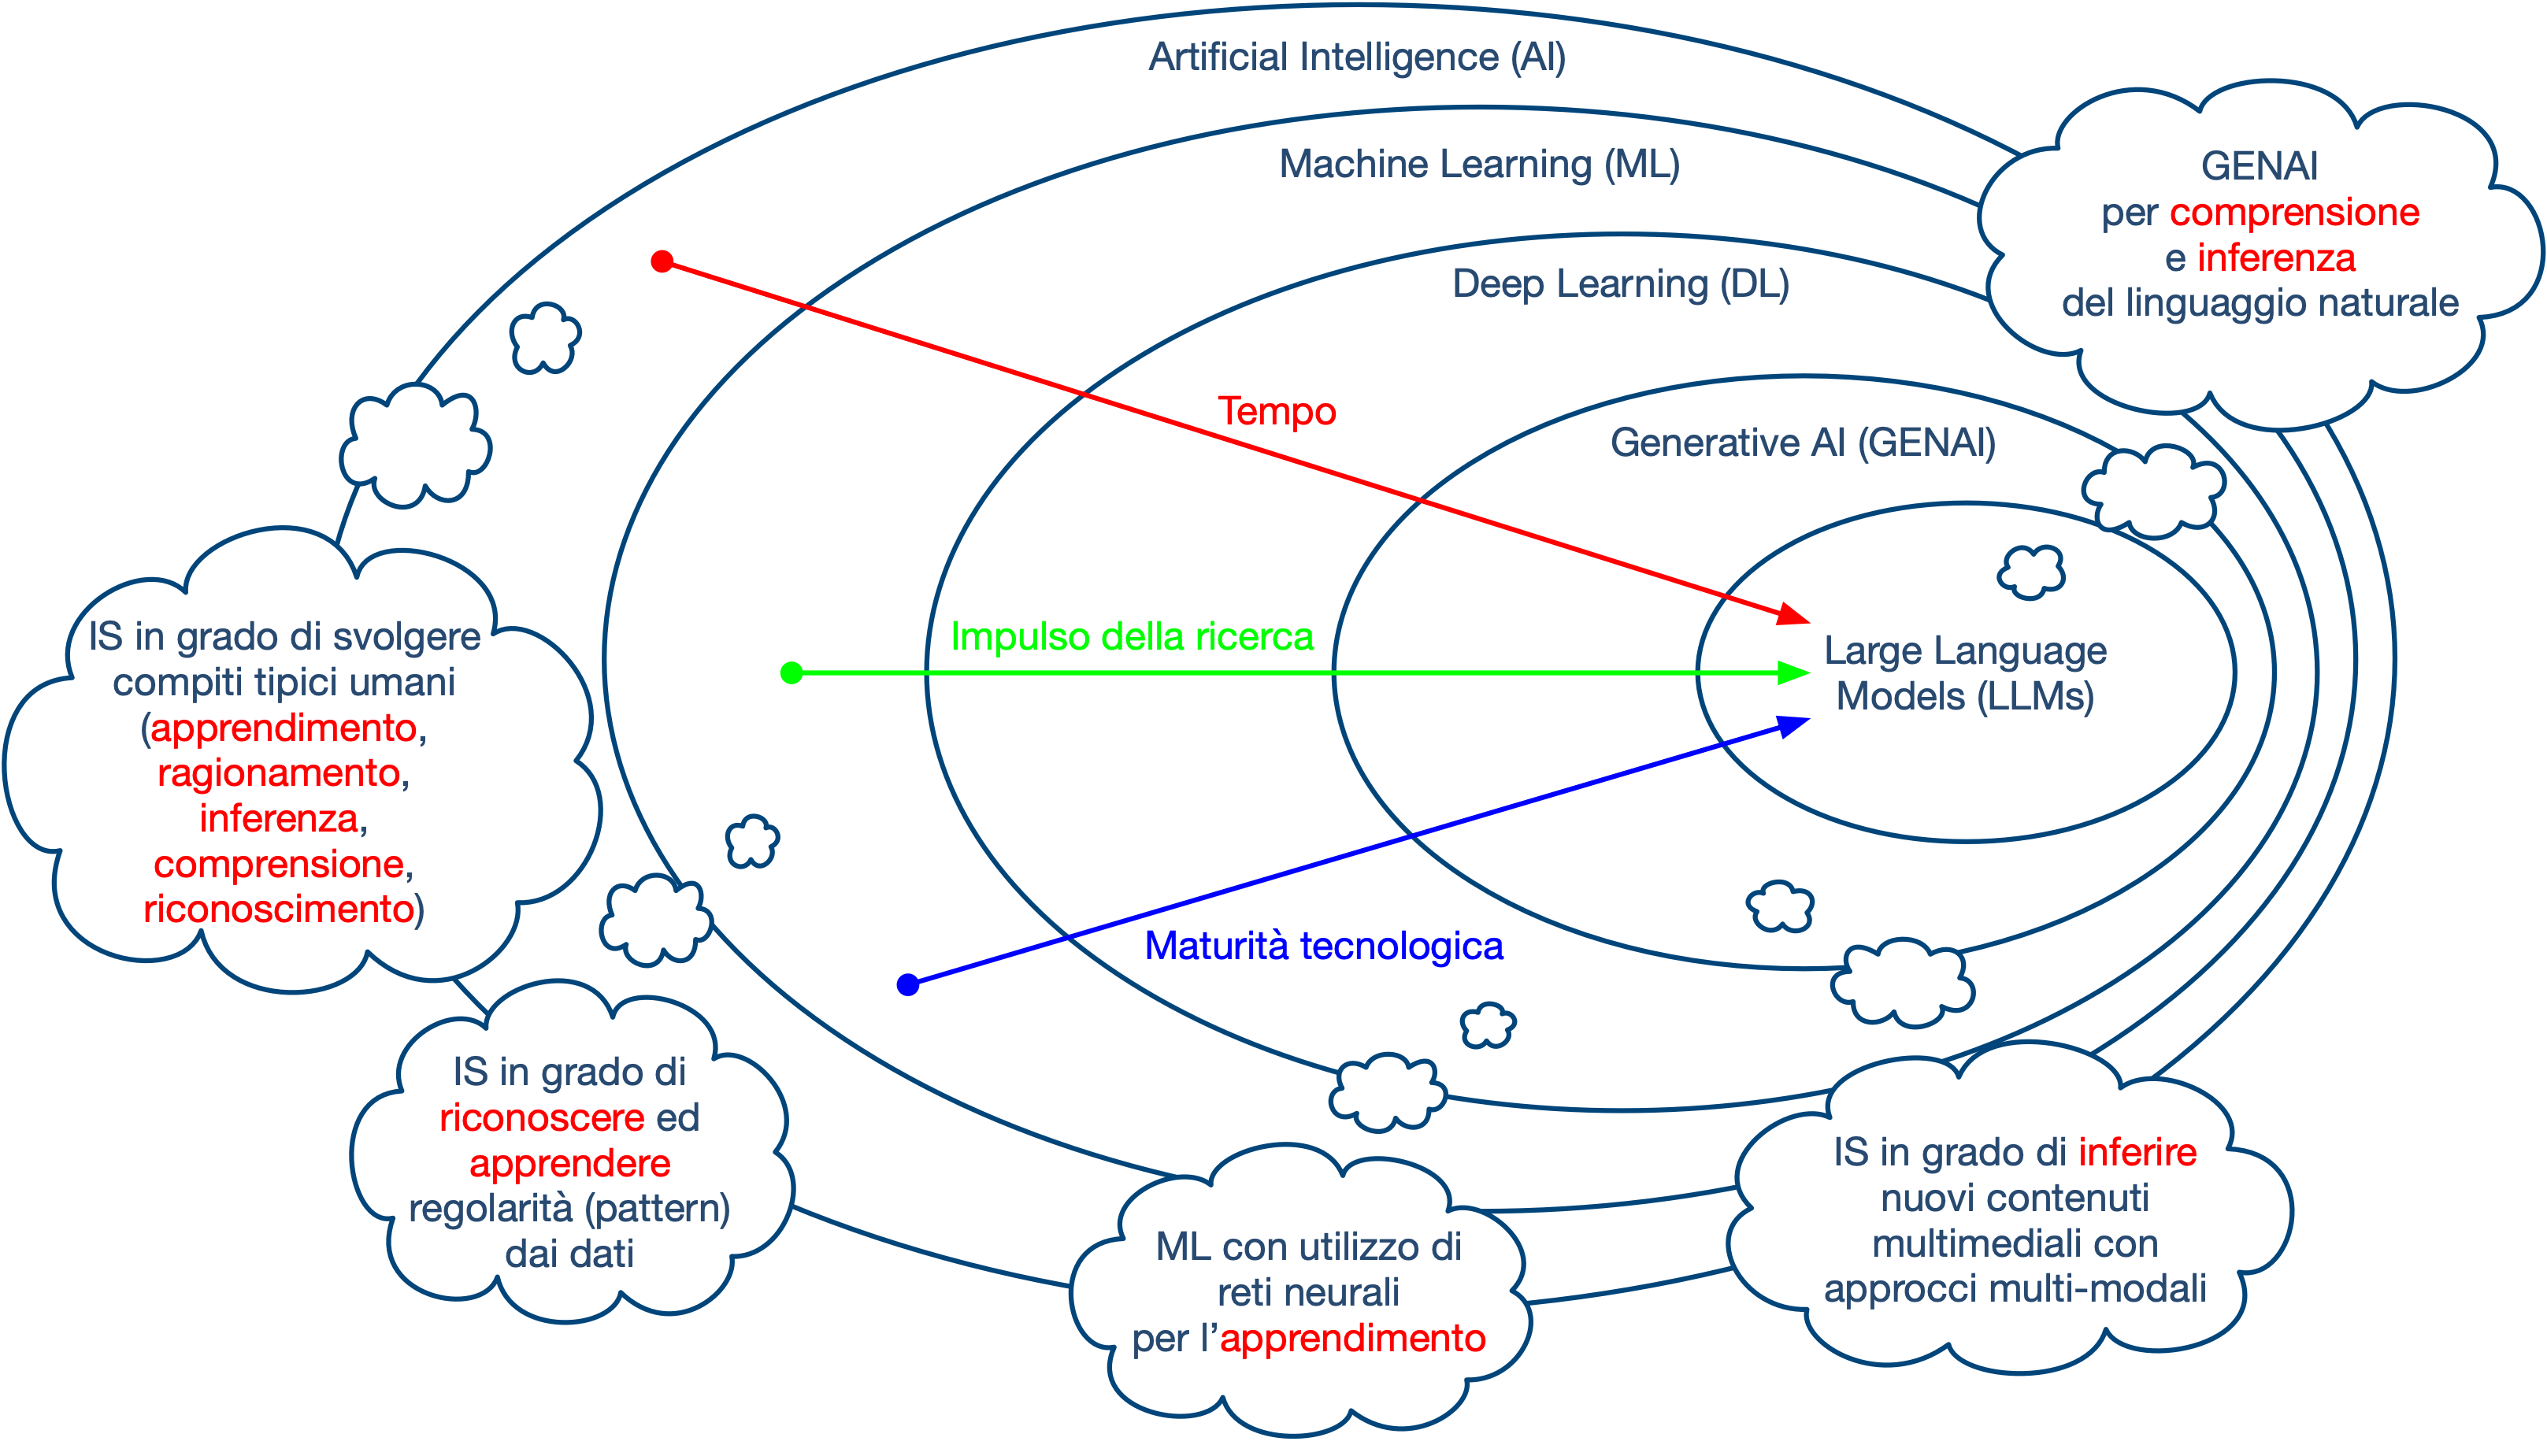
\includegraphics[width=\textwidth]{11.png}
            \end{minipage}
        \end{figure}
        }
    }
\end{frame}
%
\begin{frame}[fragile] \frametitle{Quanto?}
	\framesubtitle{Argomenti}
	{\scriptsize
	    \only<1|handout:0>{
	    \begin{figure}[ht]
                \begin{minipage}[b]{0.95\linewidth}
                    \centering
                    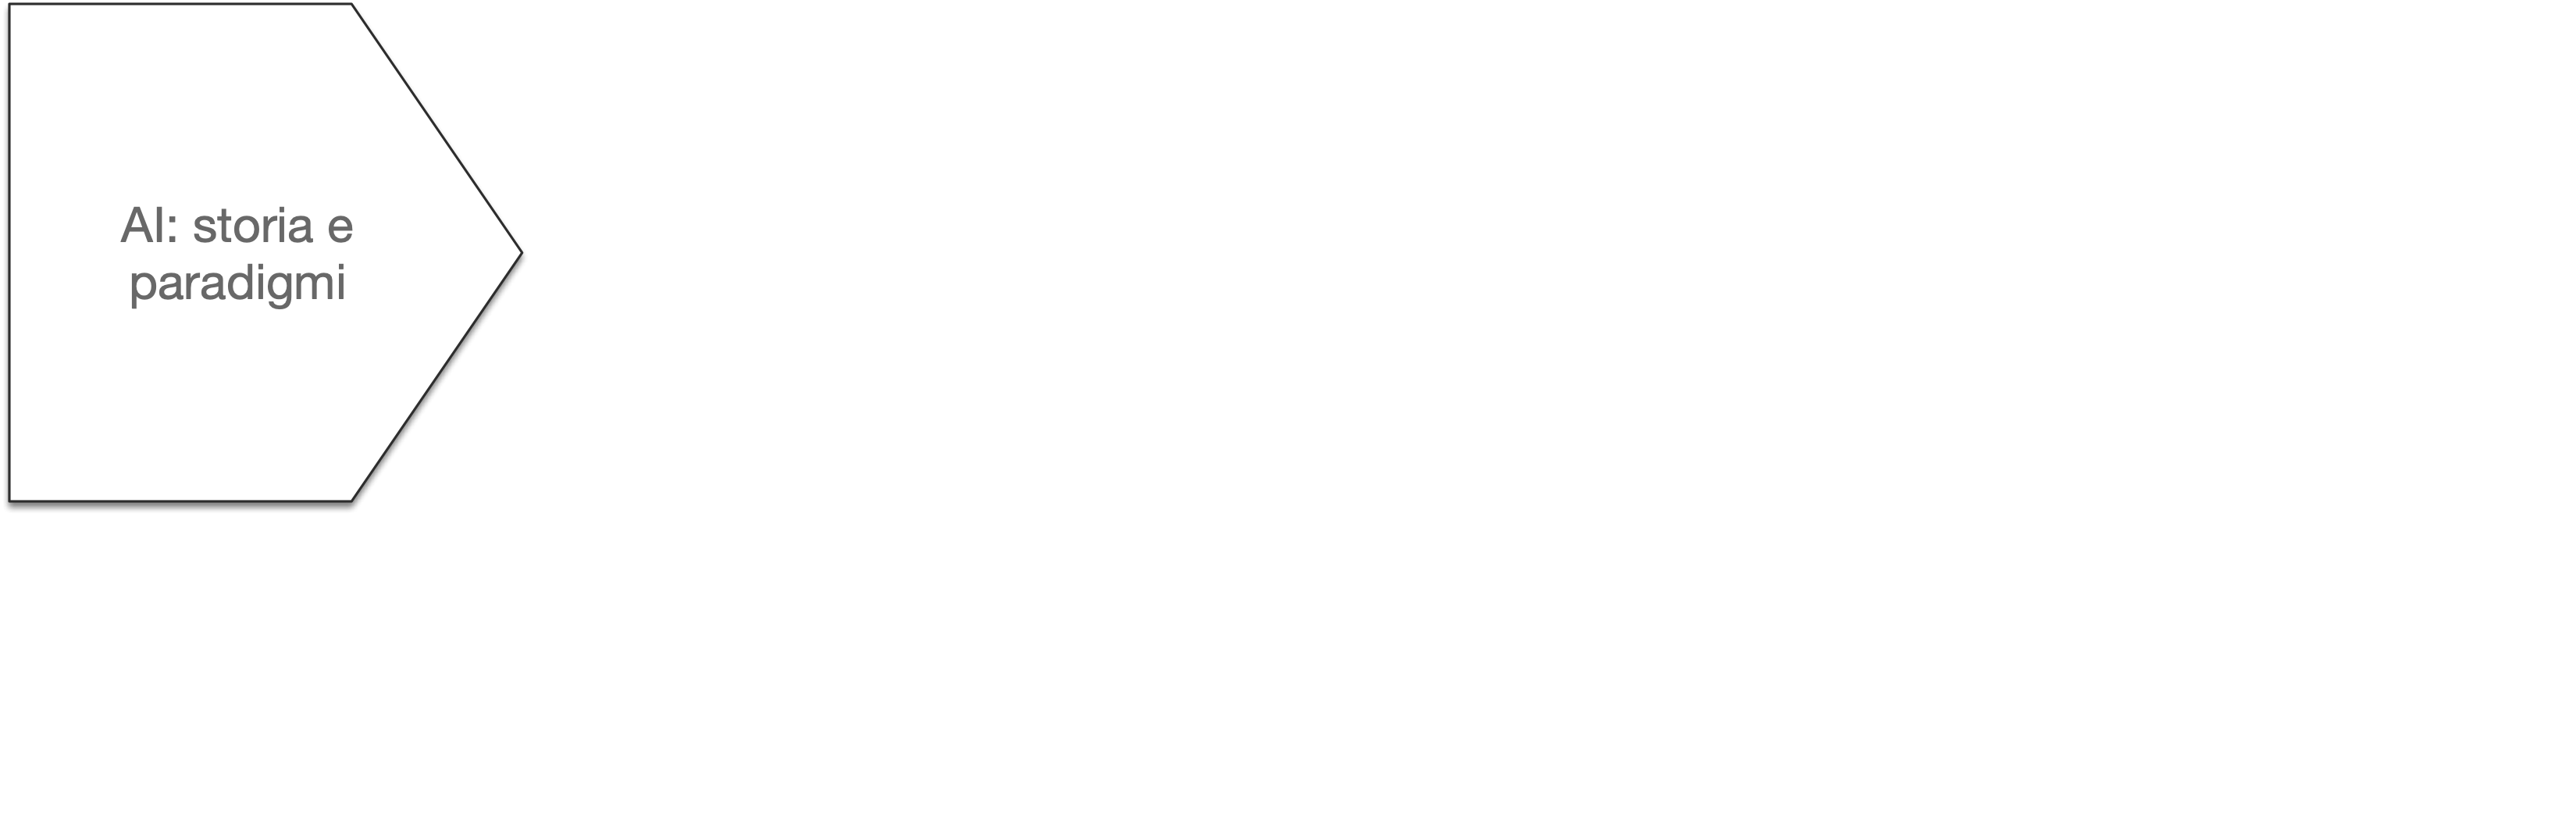
\includegraphics[width=\textwidth]{AI-house.png}
                \end{minipage}
            \end{figure}
        }
        \only<2|handout:0>{
	    \begin{figure}[ht]
                \begin{minipage}[b]{0.95\linewidth}
                    \centering
                    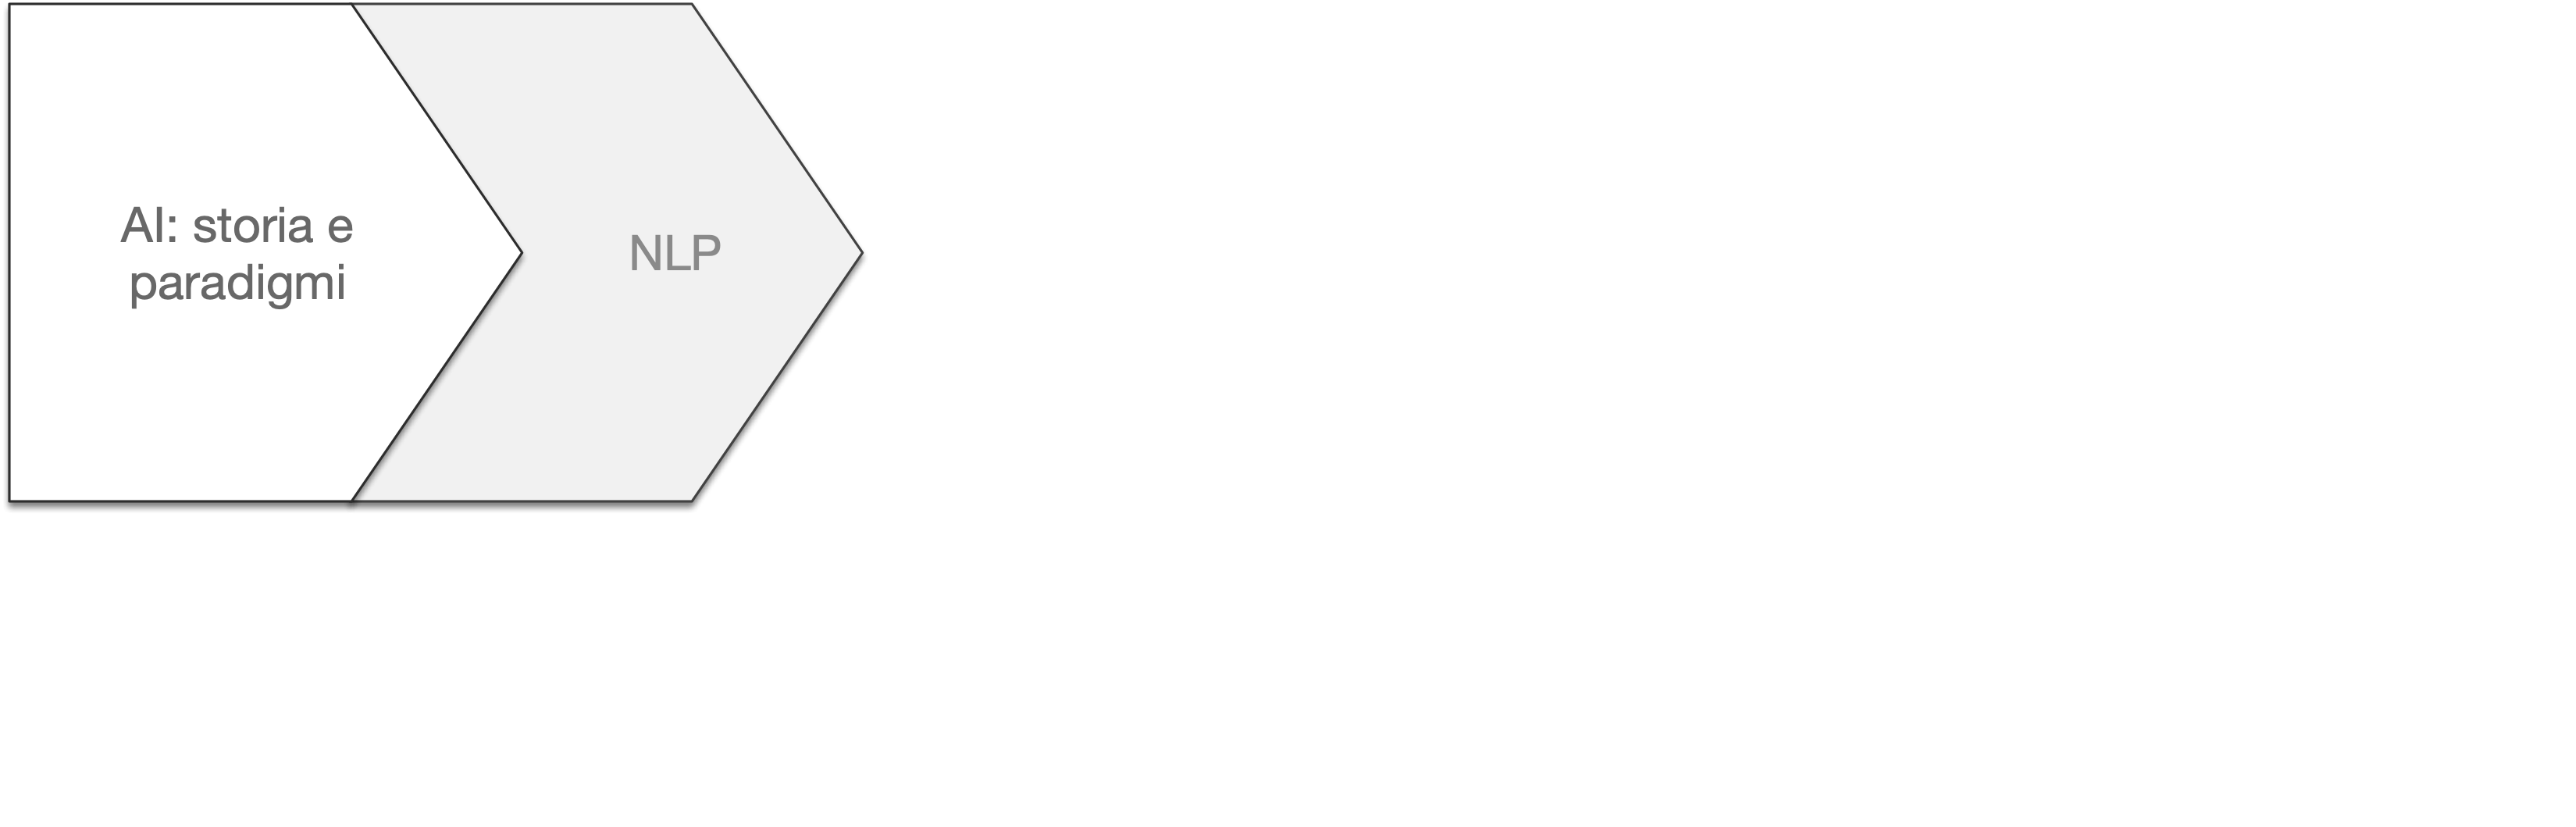
\includegraphics[width=\textwidth]{NLP-house.png}
                \end{minipage}
            \end{figure}
        }
        \only<3|handout:0>{
	    \begin{figure}[ht]
                \begin{minipage}[b]{0.95\linewidth}
                    \centering
                    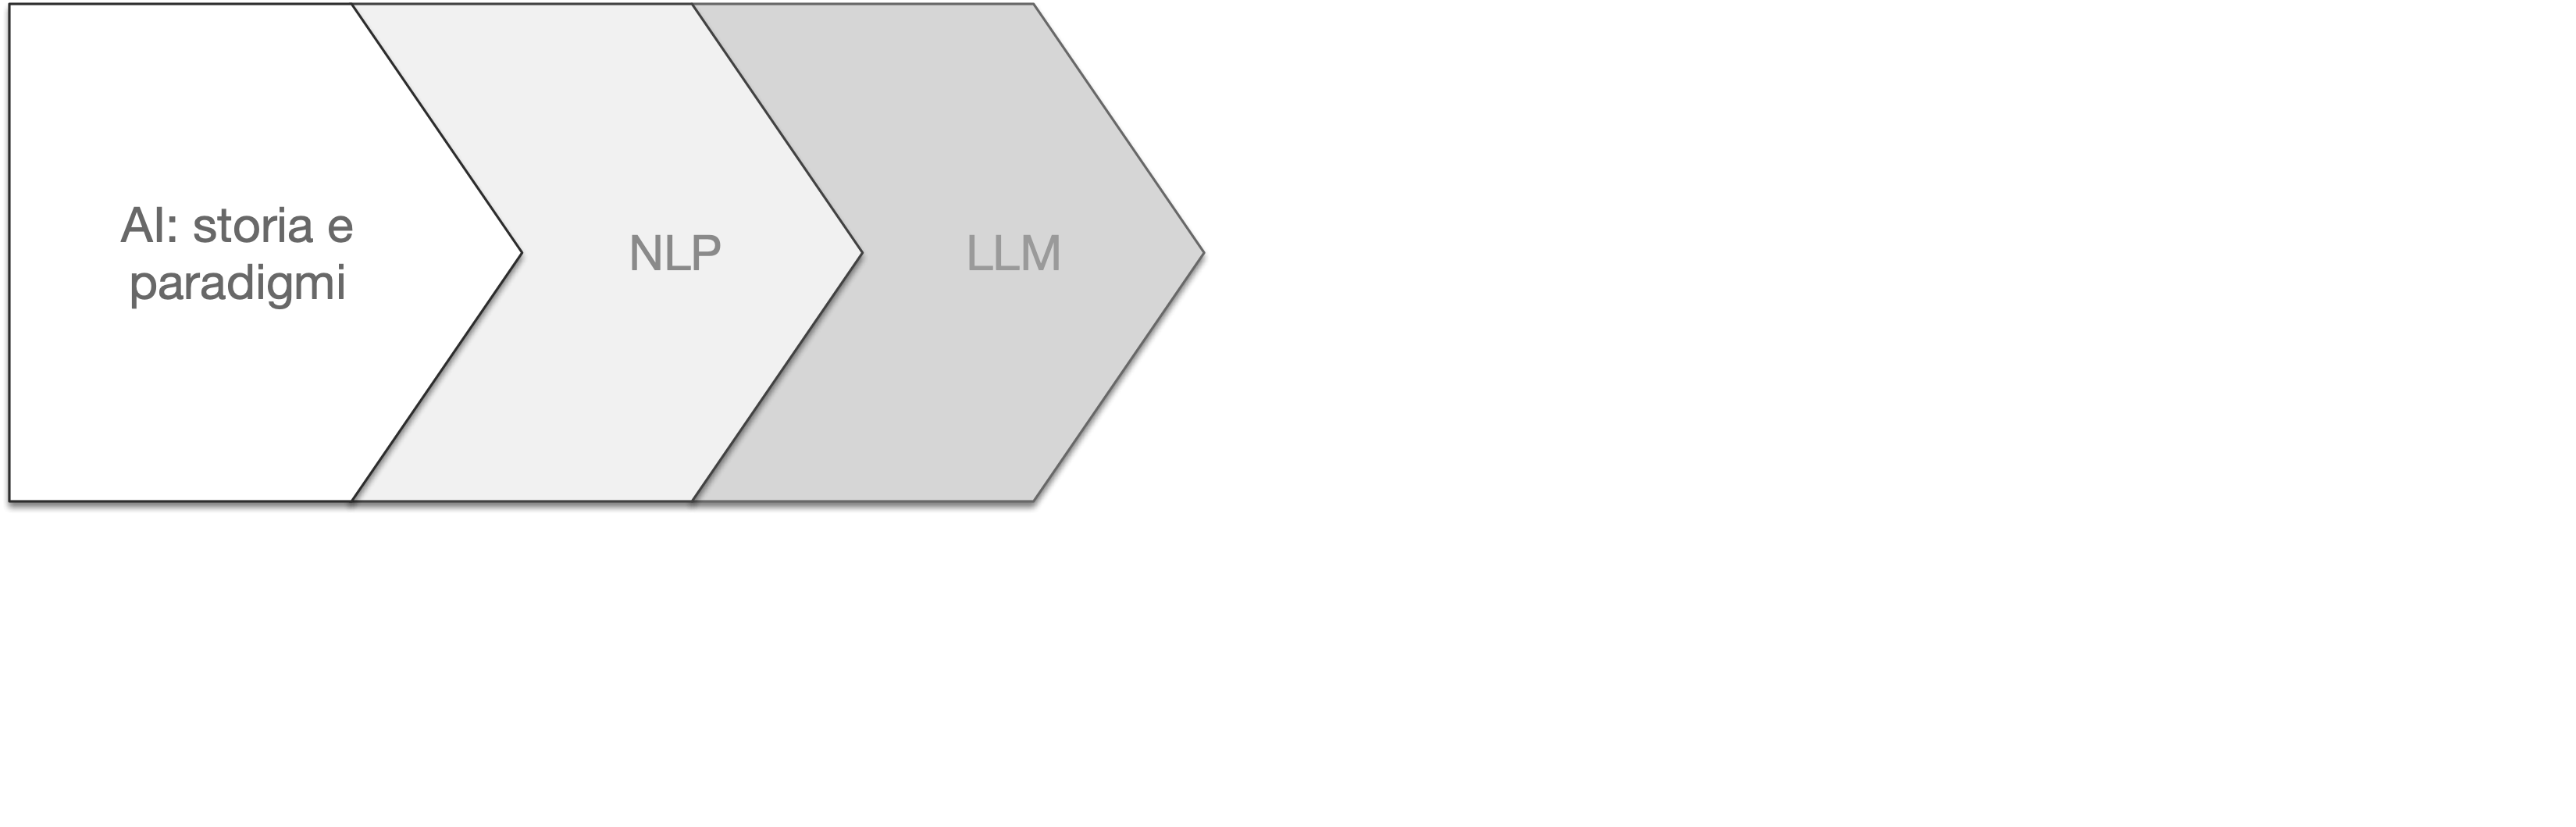
\includegraphics[width=\textwidth]{LLM-house.png}
                \end{minipage}
            \end{figure}
        }
        \only<4|handout:0>{
	    \begin{figure}[ht]
                \begin{minipage}[b]{0.95\linewidth}
                    \centering
                    
\includegraphics[width=\textwidth]{PE-house.png}
                \end{minipage}
            \end{figure}
        }
        \only<5|handout:0>{
	    \begin{figure}[ht]
                \begin{minipage}[b]{0.95\linewidth}
                    \centering
                    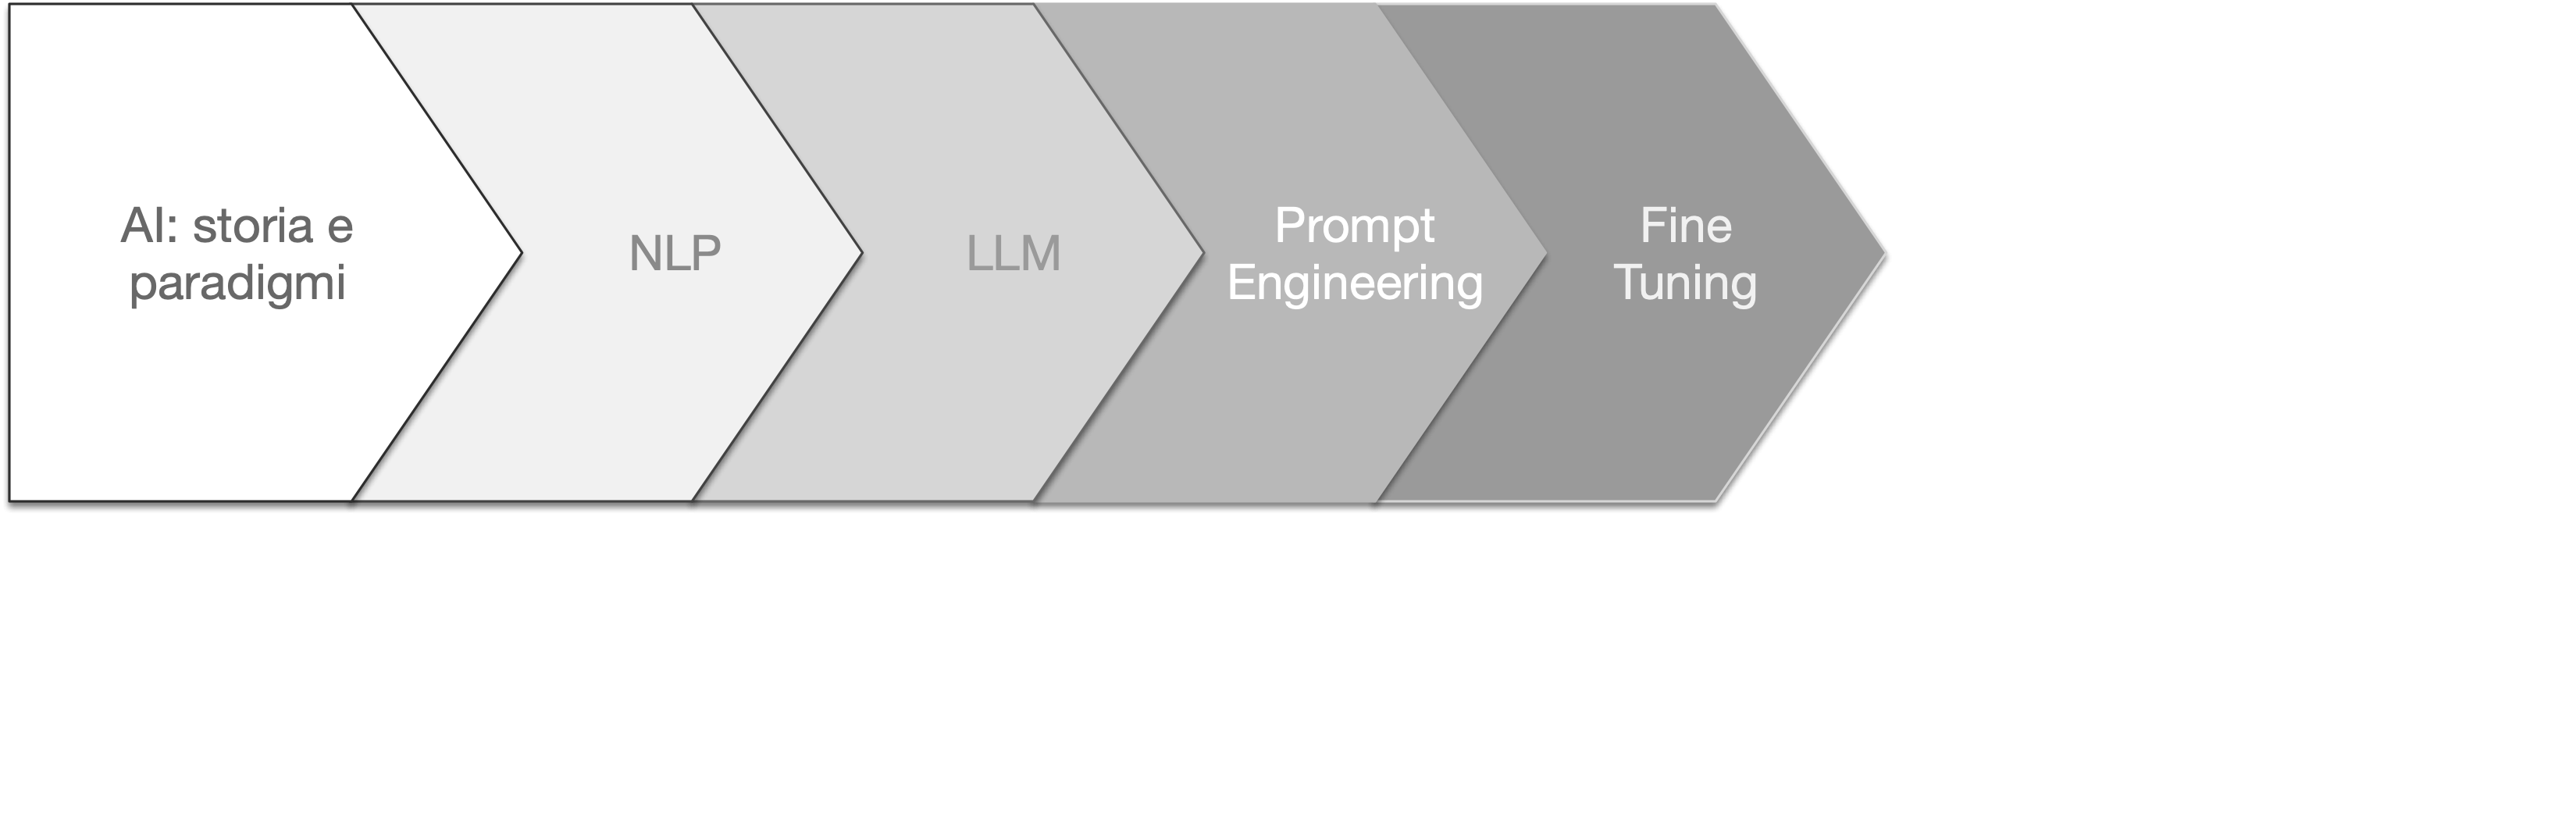
\includegraphics[width=\textwidth]{FT-house.png}
                \end{minipage}
            \end{figure}
        }
        \only<6|handout:0>{
        \begin{figure}[ht]
            \begin{minipage}[b]{0.95\linewidth}
                \centering
                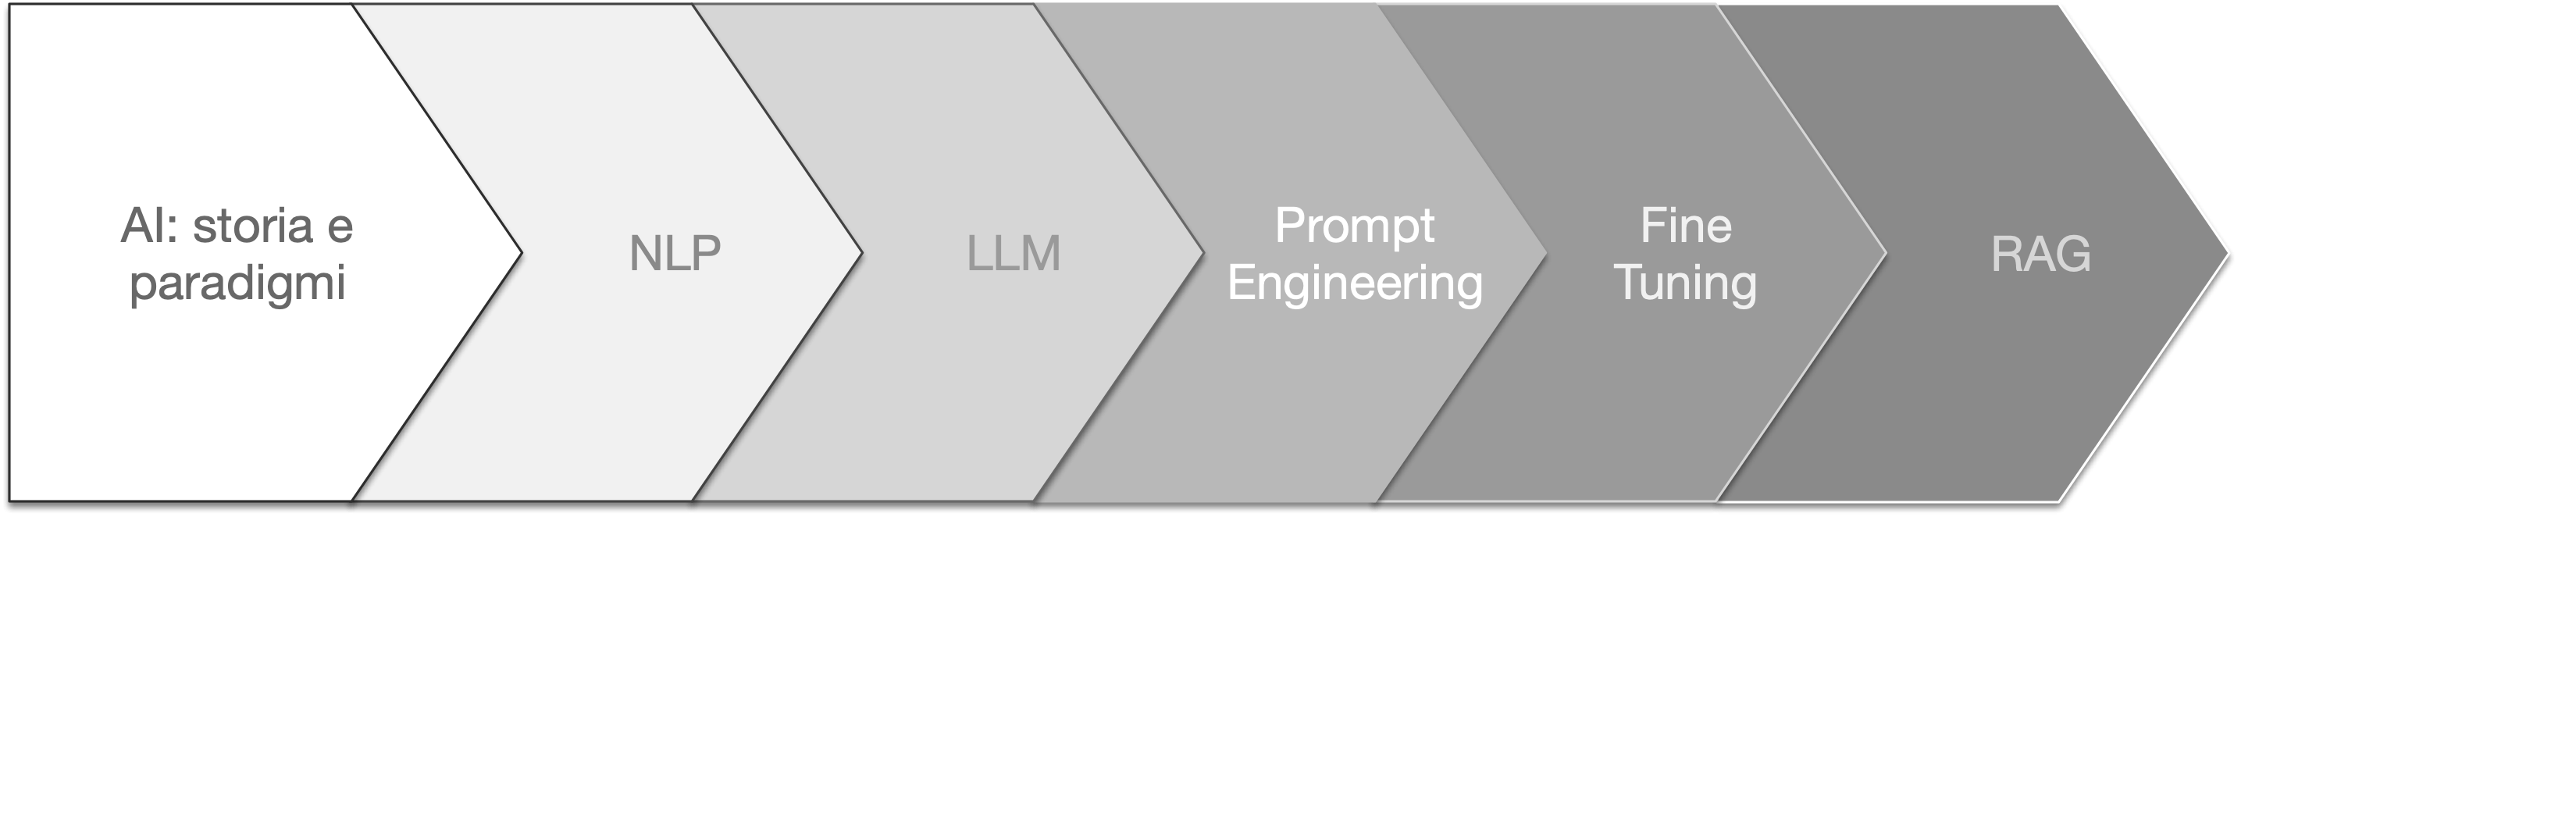
\includegraphics[width=\textwidth]{RAG-house.png}
            \end{minipage}
        \end{figure}
        }
        \only<7>{
        \begin{figure}[ht]
            \begin{minipage}[b]{0.95\linewidth}
                \centering
                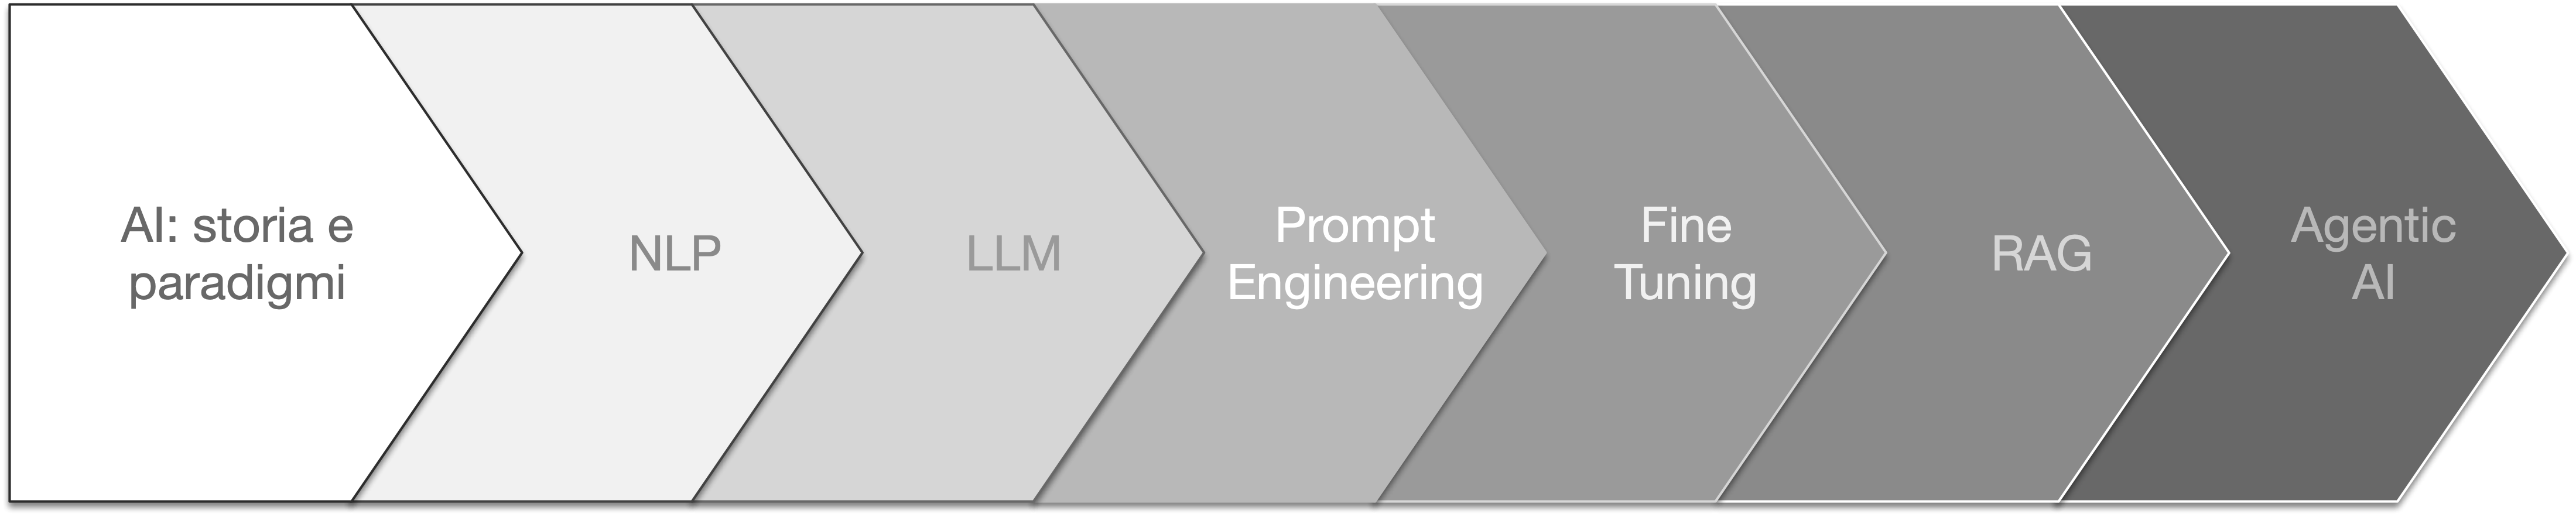
\includegraphics[width=\textwidth]{AAI-house.png}
            \end{minipage}
        \end{figure}
        }
    }
\end{frame}
%